\documentclass[a4paper,fleqn]{cas-sc}
\usepackage[authoryear,longnamesfirst]{natbib}
\usepackage{amsmath,amssymb,mathtools}
\usepackage{booktabs}
\usepackage{tabularx}
\usepackage{graphicx}
\usepackage{algorithm}
\usepackage{algpseudocode}
\algrenewcommand\alglinenumber[1]{\scriptsize #1.}
\algrenewcommand\algorithmicrequire{\textbf{Input:}}
\algrenewcommand\algorithmicensure{\textbf{Output:}}
\usepackage{float}
\usepackage{placeins}
\renewcommand{\topfraction}{0.95}
\renewcommand{\bottomfraction}{0.85}
\renewcommand{\textfraction}{0.05}
\renewcommand{\floatpagefraction}{0.75}
\setcounter{topnumber}{4}   
\setcounter{bottomnumber}{3}
\setcounter{totalnumber}{6}
\usepackage{array}
\usepackage{makecell}
\usepackage{multirow}
\usepackage{url}
\usepackage{xurl}
\usepackage{microtype}
\usepackage{adjustbox}
\definecolor{elsevierblue}{RGB}{0,112,192}
\hypersetup{
  hypertexnames=false,
  colorlinks=true,
  linkcolor=elsevierblue,
  citecolor=elsevierblue,
  urlcolor=elsevierblue
}
\renewcommand{\figurename}{Fig.}
\ExplSyntaxOn
\cs_set:Npn \__make_fig_caption:nn #1#2
{
  \l_fig_align_tl
  \skip_vertical:N \l_fig_abovecap_skip
  \setbox\cascaptionbox=\hbox{%
     \sffamily\small\textbf{\color{scolor}#1.}~#2}
  \ifdim\the\wd\cascaptionbox<\dim_use:N \l_fig_width_dim\relax
    \parbox{ \l_fig_width_dim }
      {\unskip\ignorespaces\hfil\sffamily\small
       \textbf{\color{scolor}#1.}~#2\hfil\par}
  \else
    \parbox{ \l_fig_width_dim }
      {\rightskip=0pt\unskip\ignorespaces\sffamily
       \small\textbf{\color{scolor}#1.}~#2\par}
  \fi
  \skip_vertical:N \l_fig_belowcap_skip
}
\ExplSyntaxOff
\def\tsc#1{\textsc{\lowercase{#1}}}
\newcommand{\argmax}{\operatorname*{arg\,max}}
\newcommand{\softmax}{\operatorname{Softmax}}
\newcommand{\Normalize}{\operatorname{Normalize}}
\providecommand{\figref}{}
\renewcommand{\figref}[1]{\hyperref[#1]{Fig.~\ref*{#1}}}
\providecommand{\figsref}{}
\renewcommand{\figsref}[2]{\hyperref[#1]{Figs.~\ref*{#1}--\ref*{#2}}}
\providecommand{\tabref}{}
\renewcommand{\tabref}[1]{\hyperref[#1]{Table~\ref*{#1}}}
\providecommand{\tabsref}{}
\renewcommand{\tabsref}[2]{\hyperref[#1]{Tables~\ref*{#1} and \ref*{#2}}}
\providecommand{\secref}{}
\renewcommand{\secref}[1]{\hyperref[#1]{Section~\ref*{#1}}}
\providecommand{\secsref}{}
\renewcommand{\secsref}[2]{\hyperref[#1]{Sections~\ref*{#1} and \ref*{#2}}}
\providecommand{\eqnref}{}
\renewcommand{\eqnref}[1]{\hyperref[#1]{Eq.~\eqref*{#1}}}
\begin{document}
\let\WriteBookmarks\relax
\def\floatpagepagefraction{1}
\def\textpagefraction{.001}

\shorttitle{DC-PSR for Cross-Condition Tool Wear Monitoring}
\shortauthors{Wang et~al.}
\title[mode=title]{Degradation-Consistent Probabilistic Stage Representation for Cross-Condition Tool Wear Monitoring}
\author[1,2]{Ting Wang}[orcid=0009-0006-3052-3197]
\ead{wt3377@mail.nwpu.edu.cn}
\author[1,2]{Jiali Cheng}[orcid=0009-0003-0560-2879]
\ead{chengjiali@mail.nwpu.edu.cn}
\author[1,2]{Rongze Li}[orcid=0009-0002-5787-7367]
\ead{rongzelee@mail.nwpu.edu.cn}
\author[3]{Zhenggeng Ye}[orcid=0000-0002-0636-9701]
\ead{yezhenggeng@zzu.edu.cn}
\author[4]{Keqin Wang}[orcid=0000-0001-5248-7672] 
\ead{keqinwang@nwpu.edu.cn}
\author[1,2]{Zhiqiang Cai}[orcid=0000-0002-7380-8110]
\ead{caizhiqiang@nwpu.edu.cn}
\cormark[1]
\affiliation[1]{organization={Department of Industrial Engineering, School of Mechanical Engineering, Northwestern Polytechnical University}, city={Xi'an}, postcode={710072}, country={China}}
\affiliation[2]{organization={Key Laboratory of Internet of Things-enabled Manufacturing and Quality Control Technology for Aeronautical Equipment, Ministry of Industry and Information Technology}, city={Xi'an}, postcode={710072}, country={China}}
\affiliation[3]{organization={Department of Industrial Engineering, School of Management, Zhengzhou University}, city={Zhengzhou}, postcode={450001}, country={China}}
\affiliation[4]{organization={School of Management, Northwestern Polytechnical University}, city={Xi'an}, postcode={710072}, country={China}}
\cortext[cor1]{Corresponding author}
\begin{abstract}
  Cross-condition tool wear monitoring is challenged by shifts in sensor distributions, wear scales, and stage boundaries caused by variations in cutting parameters, workpiece materials, and wear rates. These shifts make fixed-threshold labels and ordinary hard classifiers difficult to maintain consistent degradation semantics, often resulting in middle-stage compression, stage-boundary misclassification, and fluctuating probabilistic predictions. To address this problem, this paper proposes DC-PSR, a degradation-consistent probabilistic stage representation method for cross-condition tool wear monitoring. DC-PSR first constructs condition-relative stage semantics using relative degradation positions and local degradation rates, then introduces ordered fine-grained degradation states to enhance the internal structural representation of the middle stage, and finally integrates degradation-position priors, dual-side stage inhibition, and causal ordered filtering to convert instantaneous stage predictions into smoothly evolving probabilistic states along the tool life cycle. Experiments on the PHM2010 and NASA Milling datasets show that DC-PSR achieves competitive stage-discrimination performance while reducing middle-stage compression errors, suppressing non-physical stage transitions, and producing ordered stage probabilities consistent with continuous wear evolution. This study advances cross-condition tool wear stage monitoring from static categorical recognition to degradation-consistent probabilistic state representation, providing a continuously updateable state basis for tool health management under complex machining conditions.
  
\end{abstract}
\begin{keywords}
  Tool wear monitoring \sep Cross-condition generalization \sep Probabilistic stage representation \sep Degradation consistency \sep Multi-task temporal modeling
\end{keywords}
\maketitle
\section{Introduction}
\label{sec:introduction}
Tool wear monitoring is central to intelligent machining and quality control because progressive wear alters the tool-workpiece contact state and directly affects surface quality, dimensional accuracy, process stability, and production cost. Reliable representation of tool degradation from multi-source sensing signals is therefore a fundamental requirement for manufacturing health management.

With advances in multi-source sensing, deep learning, and physics-informed modeling, tool wear monitoring has moved beyond handcrafted feature extraction and single-point state recognition toward cross-condition transfer, multimodal fusion, uncertainty quantification, and hybrid prognostics. \citet{ref5} combined feature normalization, attention mechanisms, and deep learning for tool wear monitoring and multi-step prediction. \citet{ref36} introduced digital twins and contrastive learning for online wear-state representation. \citet{ref1,ref2} improved milling condition monitoring under varying cutting conditions by modeling specific cutting force coefficients and fusing direct wear observations with particle filtering. These studies show that effective tool wear monitoring requires not only recognizing the current state, but also constructing a state representation that is continuously updateable, physically consistent, and useful for downstream prediction.

This requirement becomes more challenging under cross-condition machining. Changes in cutting speed, feed rate, depth of cut, workpiece material, and tool condition simultaneously affect signal amplitudes, spectral patterns, wear growth rates, and stage boundaries. As a result, models trained under source conditions often fail to generalize to target conditions. Existing studies have addressed this issue mainly through physics-informed learning, transfer learning, domain adaptation, and multimodal fusion. Physics-informed and mechanism-guided methods have improved robustness by incorporating machining priors or mechanical coefficients \citep{ref15,ref16,ref24,ref9}. Transfer and domain adaptation methods have reduced distribution discrepancies through instance transfer, pretraining--fine-tuning, hierarchical adaptation, and frequency-domain alignment \citep{ref23,ref41,ref31,ref22}. Multimodal and uncertainty-aware methods have further enhanced wear prediction through adaptive signal processing, feature fusion, probabilistic modeling, and hybrid forecasting \citep{ref12,ref42,ref30,ref39}. Despite these advances, most studies focus on feature alignment, continuous wear prediction, or uncertainty estimation, while the semantic consistency of degradation stages across conditions remains insufficiently explored.

Wear stage is a critical intermediate representation between online monitoring and remaining useful life (RUL) prediction. Compared with a scalar wear value, a stage state provides a more interpretable indication of the tool position within its degradation life cycle and supports process stability assessment and parameter adjustment. Deep networks, graph neural networks, hidden Markov models, and clustering methods have been widely used for wear stage monitoring. Representative studies include dynamic graph isomorphism networks for multi-source stage monitoring \citep{ref3}, physics-informed and improved HMMs for wear-state transition modeling \citep{ref43,ref27}, unsupervised clustering and deep learning for stage partitioning \citep{ref32,ref26}, and acoustic-emission entropy features for revealing stage-dependent dynamics \citep{ref6}. However, these methods typically rely on fixed wear thresholds, empirical rules, or hard classification accuracy. Under cross-condition settings, absolute thresholds are easily distorted by differences in wear scale, growth rate, and failure boundary. Consequently, a model may learn condition-specific wear intervals rather than relative degradation states within the tool life cycle.

Another limitation is that hard stage classification cannot adequately represent the continuity and ordering of tool degradation. Tool wear is gradual and largely irreversible; thus, stage states should evolve from early to middle and late in an ordered manner rather than fluctuate across adjacent cuts. This issue is most critical for the middle stage. The middle stage usually covers the stable wear period, but it is not a static intermediate class. Instead, it contains a continuous internal transition from early stable wear to later accelerated degradation. With ordinary three-class supervision, the middle stage is often treated as a residual region between early and late. This may compress the stable wear period from both sides, causing samples to remain incorrectly in early, shift prematurely to late, or produce highly fluctuating stage probabilities. Recent studies have highlighted the internal structural differences, continuity, and irreversibility of tool wear processes \citep{ref40,ref20}. These observations suggest that cross-condition stage modeling should move beyond macro-level hard labels toward probabilistic stage representation with relative degradation semantics, internal stage structure, and temporal ordering constraints.

Multi-task learning, physical constraints, and probabilistic inference provide useful foundations for such representation. Multi-task learning can enhance degradation perception through shared representations across related tasks, such as joint modeling of tool wear and breakage, surface quality, or roughness prediction \citep{ref19,ref18,ref10,ref34}. \citet{ref13} improved industrial anomaly detection using multi-stage one-class learning. Physical constraints and mechanism-driven models have further improved the consistency and interpretability through probabilistic state-space fusion, mechanism-driven data modeling, filtering-based estimation, online calibration, and physics-informed learning frameworks \citep{ref17,ref28,ref7,ref8,ref29,ref38}. In addition, \citet{ref14} connected stage recognition, SVR, and particle filtering for wear prediction, showing that stage information can serve as a useful preceding state for prognostics. Nevertheless, existing studies mostly treat stage information as a label, auxiliary variable, or preprocessing result. A continuous, ordered, and interpretable probabilistic stage representation for cross-condition tool wear monitoring remains underdeveloped.

To address this gap, this paper argues that cross-condition wear stage representation should satisfy three requirements. First, stage definitions should avoid dependence on fixed absolute thresholds and preserve relative degradation semantics across conditions. Second, the model should characterize the fine-grained internal structure of the middle stage to prevent compression of the stable wear period. Third, the output should not be a single hard label, but a probabilistic stage state that evolves smoothly and monotonically along the tool life cycle. Motivated by these requirements, this paper proposes a degradation-consistent probabilistic stage representation method, termed DC-PSR. The proposed method constructs relative stage semantics using relative degradation positions and local degradation rates, enhances middle-stage representation through ordered fine-grained degradation states, and integrates degradation-position priors, dual-side stage inhibition, and causal ordered filtering to generate degradation-consistent probabilistic stage states.

The main contributions of this paper are summarized as follows.

(1) A degradation-consistent probabilistic stage representation framework is proposed for cross-condition tool wear monitoring. Instead of fixed wear thresholds, the framework uses condition-relative degradation states and online relative features to reduce signal-scale drift and stage-related representation bias, preserving consistent life-cycle semantics across conditions.

(2) A fine-grained-state-assisted multi-task temporal model is developed. Ordered fine-grained substates are constructed in the relative degradation space and jointly learned with macro-stage classification and continuous degradation-position estimation via TCN-GRU. This design enables the model to capture both stage boundaries and the internal hierarchy of the middle stage.

(3) A degradation-consistent probabilistic inference mechanism is designed. By integrating raw stage probabilities, fine-state cues, and degradation-position priors with dual-side inhibition and causal ordered filtering, the mechanism suppresses non-physical stage transitions and converts instantaneous stage decisions into smoothly evolving probabilistic states along the tool life cycle.

The remainder of this paper is organized as follows. \secref{sec:problem} formulates the problem and presents the overall framework. \secref{sec:method} introduces the proposed method. \secref{sec:experiments} describes the datasets, experimental settings, and evaluation metrics. \secref{sec:results} reports the experimental results. \secref{sec:discussion} discusses the effectiveness, applicability, and limitations. \secref{sec:conclusions} concludes the paper.

\section{Problem Formulation}
\label{sec:problem}
An ideal probabilistic stage representation for tool wear monitoring should satisfy three requirements: semantic consistency across conditions, separability of the middle-stage structure, and ordered evolution of stage probabilities. Accordingly, stage monitoring is formulated as a probabilistic state representation problem rather than a single-point classification task.

Let $\mathbf{X}_{c,t}$ denote the input feature window of the $t$-th cut under condition $c$. The objective is to estimate the probability distribution of the current tool state over three macro wear stages:
\begin{equation}
  \begin{aligned}
    \mathbf{p}_{c,t}^{\mathrm{final}}=[p_{c,t}^{\mathrm{final},E},p_{c,t}^{\mathrm{final},M},p_{c,t}^{\mathrm{final},L}]
  \end{aligned}
\end{equation}
where $E$, $M$, and $L$ denote the early, middle, and late stages, corresponding to the initial wear, stable wear, and accelerated wear stages, respectively. Unlike a hard label, $\mathbf{p}_{c,t}^{\mathrm{final}}$ not only identifies the most likely current stage, but also characterizes the continuous evolution of stage confidence along the degradation process, especially the transition uncertainty and stage-related reliability near stage boundaries.

The overall framework of DC-PSR is shown in \figref{fig:1}. It contains three coupled components: relative stage semantics, fine-grained degradation states, and ordered probabilistic inference. Relative stage semantics alleviate cross-condition shifts in degradation scale and stage boundaries. Fine-grained states enhance the internal representation of the middle stage. The TCN-GRU network and ordered probabilistic inference provide instantaneous stage discrimination and life-cycle consistency constraints, respectively.

\begin{figure}[pos=!htbp]
  \centering
  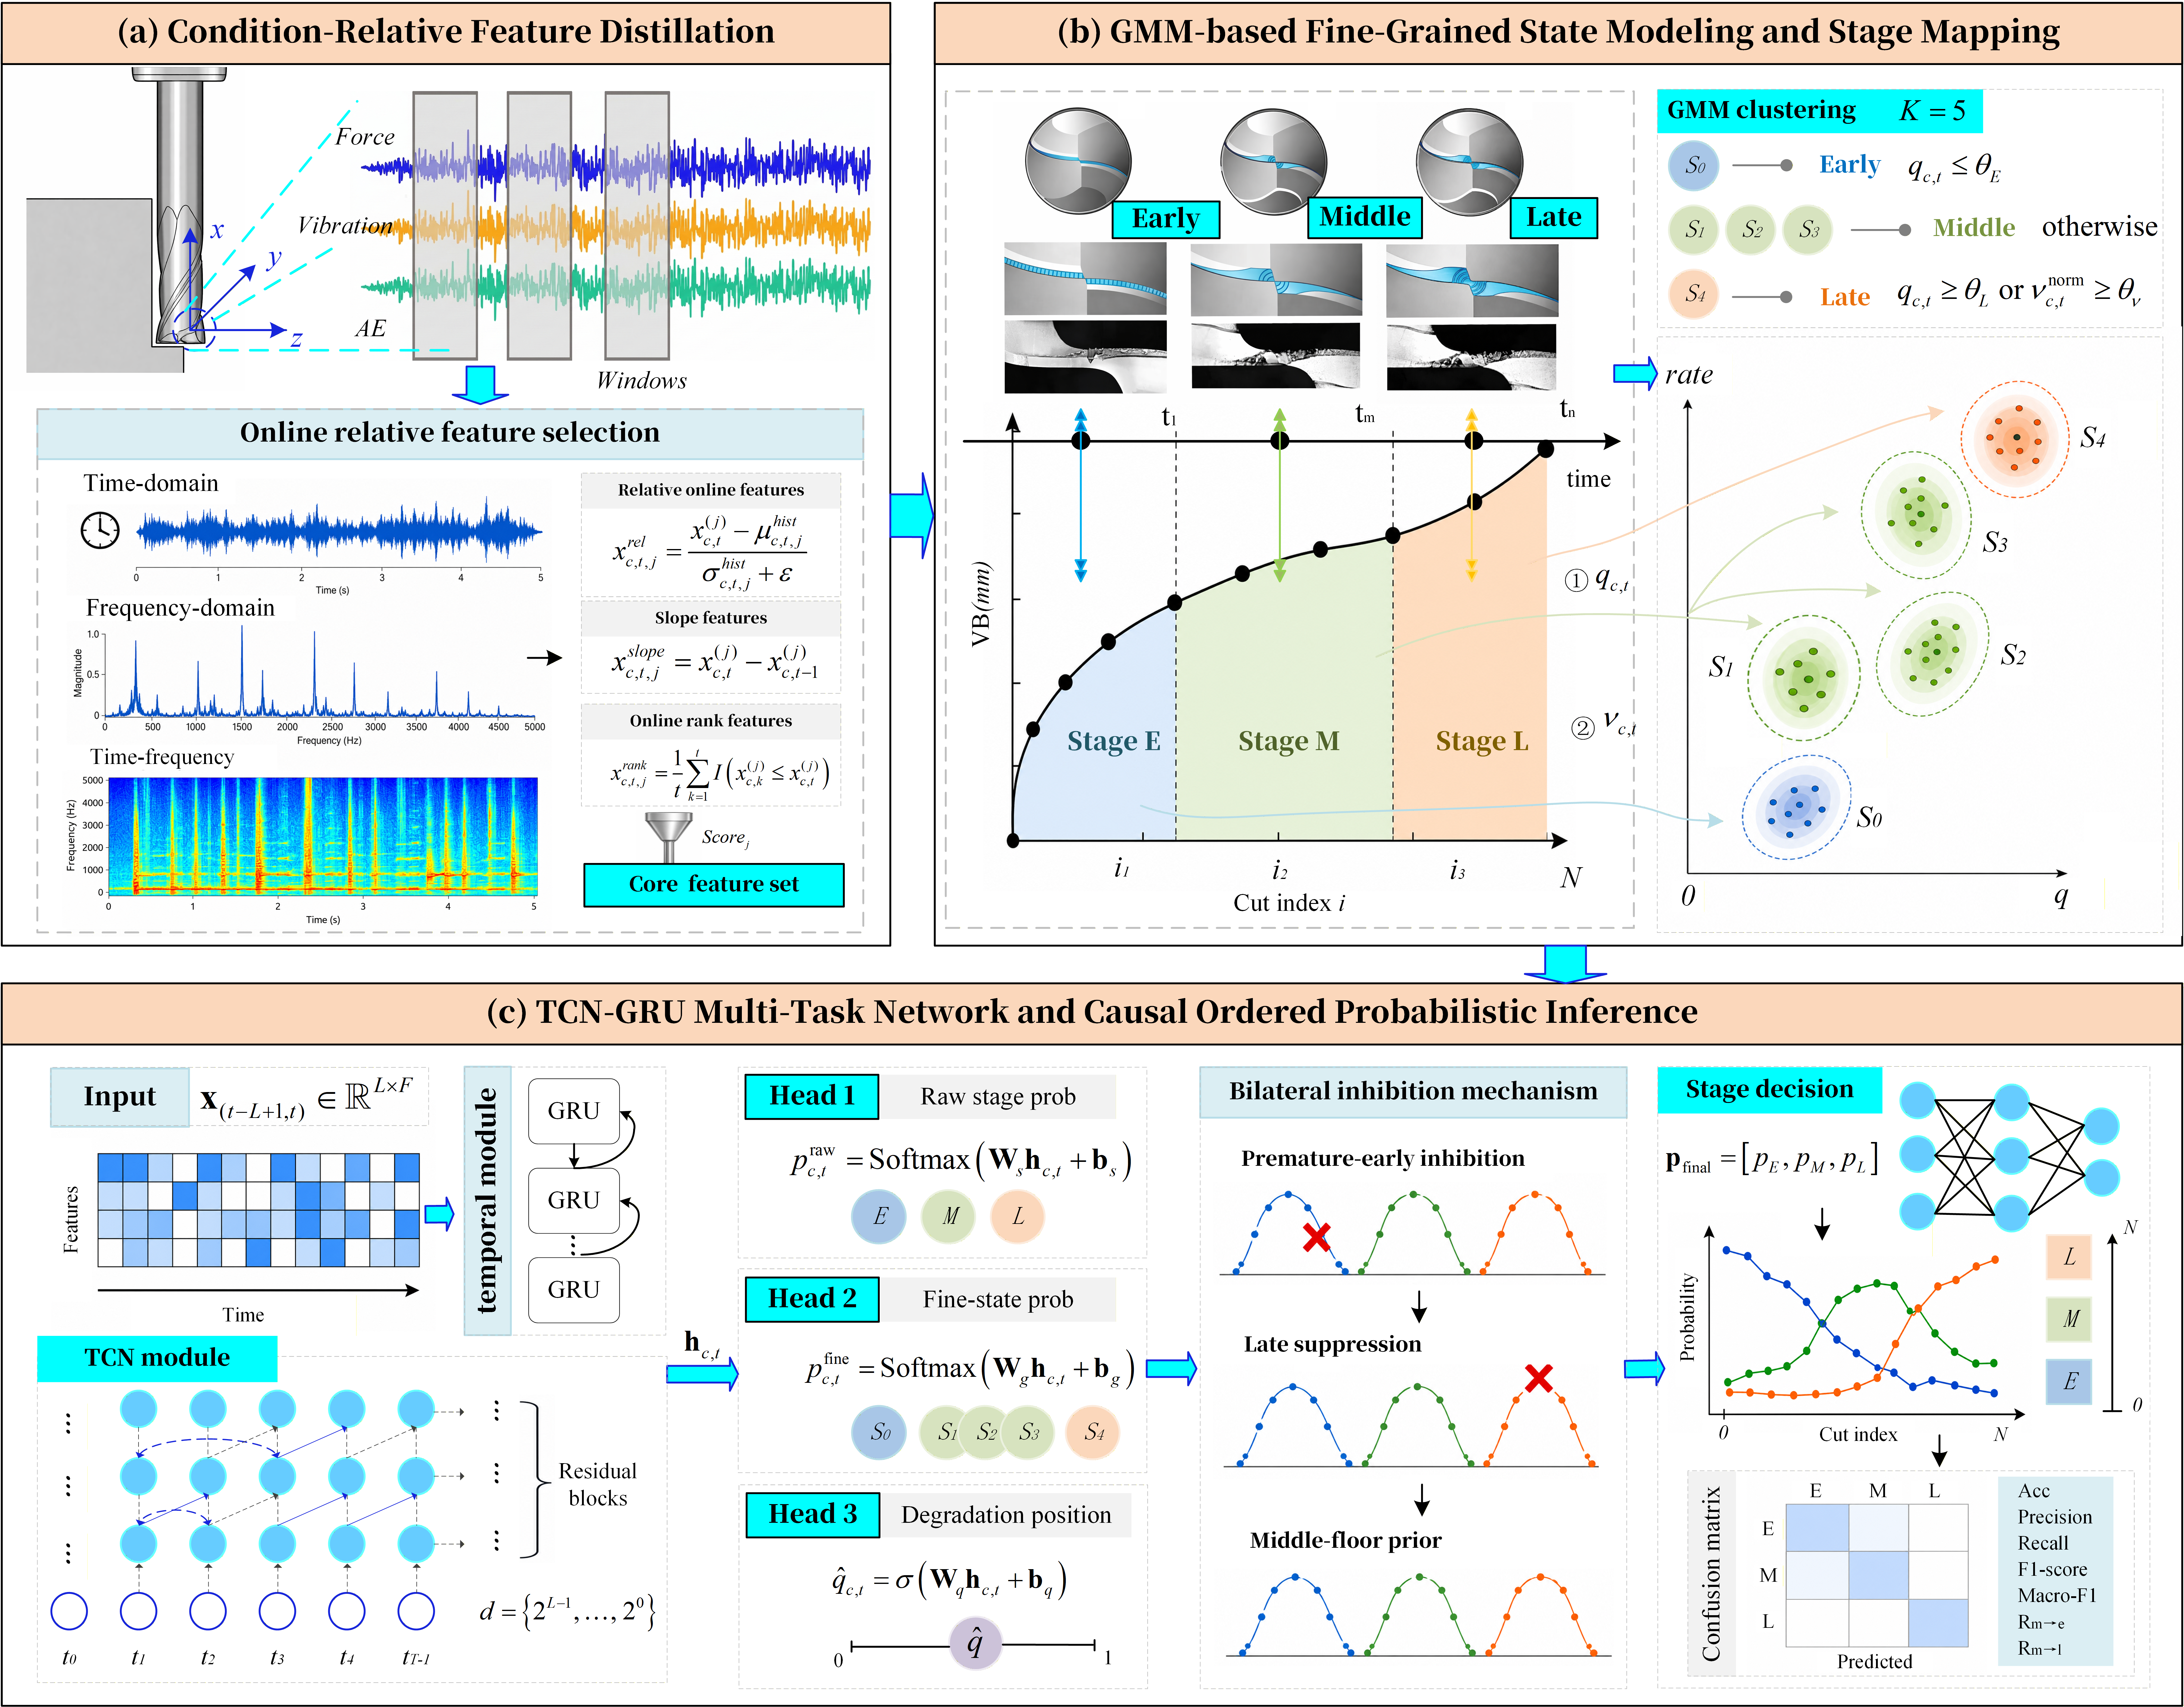
\includegraphics[width=\textwidth,keepaspectratio]{figures/fig1.png}
  \caption{Overall framework of DC-PSR.}
  \label{fig:1}
\end{figure}
Through this formulation, DC-PSR converts stage monitoring into probabilistic state modeling under multiple degradation constraints, enabling the output to represent both stage likelihood and degradation-order consistency. The main symbols used in this paper are summarized in \tabref{tab:1}.

\begin{table}[!htbp]
  \centering
  \scriptsize
  \caption{Main symbols and definitions.}
  \label{tab:1}
  \begin{adjustbox}{max width=\textwidth}
    \begin{tabular}{llll}
      \toprule
      \textbf{Symbol} & \textbf{Definition} & \textbf{Symbol} & \textbf{Definition} \\
      \midrule
      $c$ & Cutting condition & $t$ & Cut index \\
      $VB_{c,t}$ & Flank wear & $\widetilde{VB}_{c,t}$ & Smoothed flank wear \\
      $q_{c,t}$ & Relative degradation position & $\nu_{c,t}^{\mathrm{norm}}$ & Normalized local wear rate \\
      $s_{c,t}$ & Macro-stage label & $g_{c,t}$ & Fine-grained state \\
      $\mathbf{x}_{c,t}$ & Feature vector & $\mathbf{X}_{c,t}$ & Sliding window \\
      $\mathbf{p}_{c,t}^{\mathrm{raw}}$ & Raw stage probability & $\mathbf{p}_{c,t}^{g}$ & Fine-state probability \\
      $\mathbf{p}_{c,t}^{\mathrm{fine}}$ & Fine-derived stage probability & $\hat{q}_{c,t}$ & Estimated degradation position \\
      $\mathbf{p}_{c,t}^{\mathrm{prior}}$ & Position-prior probability & $\mathbf{p}_{c,t}^{\mathrm{mix}}$ & Mixed stage probability \\
      $\boldsymbol{\alpha}_{c,t}$ & Ordered stage probability & $\mathbf{p}_{c,t}^{\mathrm{final}}$ & Final stage probability \\
      $\eta$ & Raw-probability weight & $\omega_{f}$ & Fine-probability weight \\
      $\beta$ & Ordered-probability weight & $\theta_{E},\theta_{L},\theta_{\nu}$ & Stage thresholds \\
      \bottomrule
    \end{tabular}
    \end{adjustbox}
\end{table}

\section{Proposed Method}
\label{sec:method}
The objective of DC-PSR is to transform cross-condition tool wear stage monitoring from discrete category discrimination into degradation-consistent probabilistic state representation. Accordingly, DC-PSR is developed through three components: condition-relative stage semantics, fine-grained degradation state modeling, and ordered probabilistic inference.

\subsection{Condition-Relative Stage Semantics}
\label{sec:stage_semantics}
To maintain consistent degradation semantics across conditions, a condition-relative degradation scale is first constructed. Let $VB_{c,t}$ be the flank wear of the $t$-th cut under condition $c$. After smoothing the wear sequence as $\widetilde{VB}_{c,t}$, the relative degradation position is defined as
\begin{equation}
  \begin{aligned}
    q_{c,t} =
    \frac{
    \widetilde{VB}_{c,t}-\min(\widetilde{VB}_{c})
    }{
    \max(\widetilde{VB}_{c})-\min(\widetilde{VB}_{c})+\varepsilon
    }
  \end{aligned}
\label{eq:q_true}
\end{equation}
where $q_{c,t}\in [0,1]$ denotes the relative position of the current tool within its condition-specific life cycle, and $\varepsilon$ is a small constant. The local degradation rate is computed from the first-order difference of $q_{c,t}$:
\begin{equation}
  \begin{aligned}
    \nu_{c,t}=q_{c,t}-q_{c,t-1}
  \end{aligned}
\label{eq:local_rate}
\end{equation}
and then smoothed and normalized as $\nu_{c,t}^{\mathrm{norm}}$. Here, $q_{c,t}$ represents the degradation position, while $\nu_{c,t}^{\mathrm{norm}}$ reflects the local acceleration of wear. The macro-stage label is assigned by
\begin{equation}
	s_{c,t} =
	\begin{cases}
		E, & q_{c,t}\le \theta_E,\\
		L, & q_{c,t}\ge \theta_L \ \text{or}\ \nu_{c,t}^{\mathrm{norm}}\ge \theta_\nu,\\
		M, & \text{otherwise}.
	\end{cases}
	\label{eq:stage_label}
\end{equation}
  where $s_{c,t}\in \{E,M,L\}$. The thresholds $\theta_{E}$, $\theta_{L}$, and $\theta_{\nu}$ are determined by condition-specific quantiles:
  \begin{equation}
    \begin{aligned}
      Q_{E}=0.30,Q_{L}=0.72,Q_{\nu}=0.78
    \end{aligned}
  \end{equation}
  
  \figref{fig:2} shows that stage boundaries vary across conditions, supporting the need to describe tool states using relative degradation positions rather than fixed absolute wear thresholds.

  \begin{figure}[pos=!htbp]
    \centering
    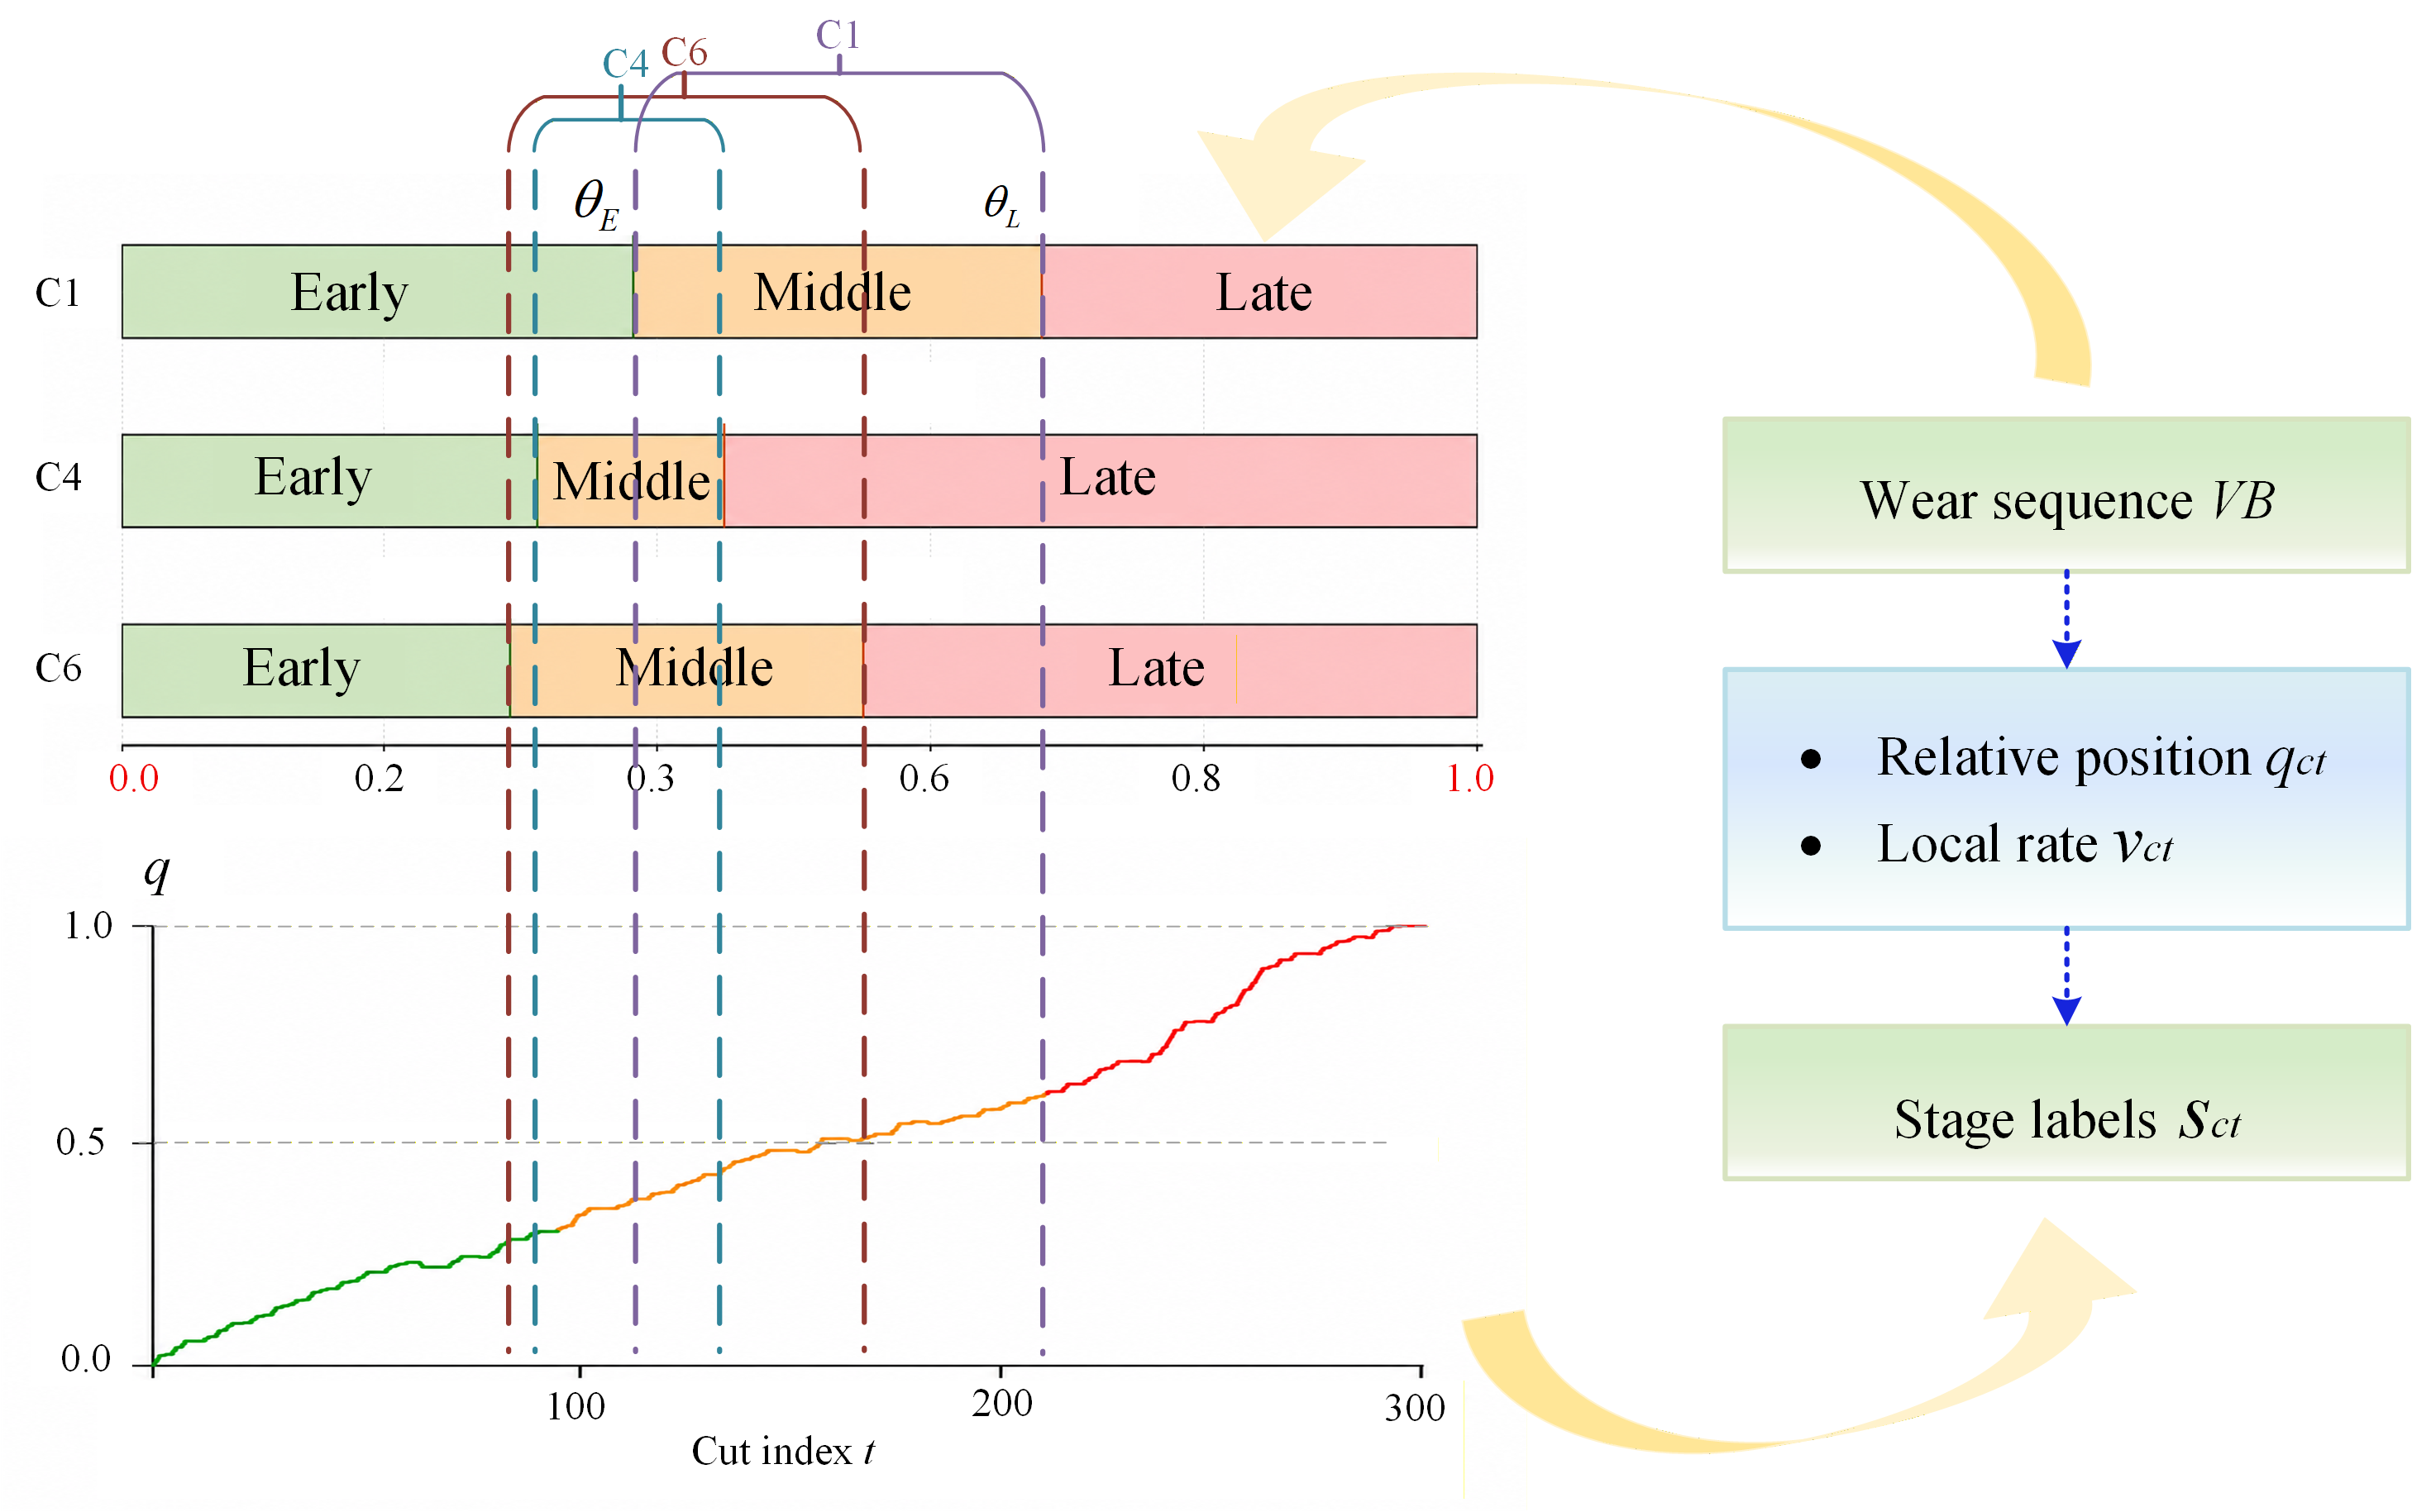
\includegraphics[width=0.62\textwidth,keepaspectratio]{figures/fig2.png}
    \caption{Condition-relative stage partitioning.}
    \label{fig:2}
  \end{figure}
Although relative stage semantics reduce label-level inconsistency, sensing features may still suffer from cross-condition scale drift. Therefore, online condition-relative features are constructed using only current and historical observations. For the $j$-th raw sensing feature $x_{c,t}^{\left(j\right)}$, three online features are extracted.

  First, the online relative standardized feature is defined as
  \begin{equation}
    \begin{aligned}
      x_{c,t,j}^{rel}=\frac{x_{c,t}^{\left(j\right)}-\mu_{c,t,j}^{hist}}{\sigma_{c,t,j}^{hist}+\varepsilon}
    \end{aligned}
  \end{equation}
  where $\mu_{c,t,j}^{hist}$ and $\sigma_{c,t,j}^{hist}$ are computed from observations $1,\ldots,t$ under the current condition only. This feature measures the deviation of the current observation from its historical distribution.

  Second, the local variation feature is defined as
  \begin{equation}
    \begin{aligned}
      x_{c,t,j}^{slope}=x_{c,t}^{\left(j\right)}-x_{c,t-1}^{\left(j\right)}
    \end{aligned}
  \end{equation}
  which captures the short-term change of the feature between adjacent cuts.

  Third, the online relative rank feature is defined as
  \begin{equation}
    \begin{aligned}
      x_{c,t,j}^{\mathrm{rank}}
      =
      \frac{1}{t}\sum_{k=1}^{t}
      I\!\left(x_{c,k}^{(j)}\le x_{c,t}^{(j)}\right)
    \end{aligned}
  \end{equation}
  where $I(\cdot )$ is the indicator function. It represents the relative rank of the current observation among historical samples of the same condition.

  To select features that are both degradation-relevant and cross-condition stable, a comprehensive score is designed by combining stage discriminability, degradation relevance, monotonicity, and distribution stability. Inspired by \citet{ref4}, \citet{ref11}, and \citet{ref25}, the score of feature $x_{j}$ is defined as
  \begin{equation}
    \begin{aligned}
      Score_{j}=\alpha_{1}MI(x_{j},s)+\alpha_{2}MI(x_{j},q)+\alpha_{3}|\rho(x_{j},q)|-\alpha_{4}DI_{j}
    \end{aligned}
  \end{equation}
  where $MI(x_{j},s)$ measures stage discriminability, $MI(x_{j},q)$ measures degradation relevance, $|\rho(x_{j},q)|$ is the absolute Spearman correlation coefficient, and $DI_{j}$ measures distribution instability across training conditions. Taking C1 and C4 as an example,
  \begin{equation}
    \begin{aligned}
      DI_{j}=\frac{|\mu_{C1,j}-\mu_{C4,j}|}{0.5(\sigma_{C1,j}+\sigma_{C4,j})+\varepsilon}
    \end{aligned}
  \end{equation}
  where $\mu_{C1,j}$, $\mu_{C4,j}$, $\sigma_{C1,j}$, and $\sigma_{C4,j}$ are the means and standard deviations of $x_{j}$ under C1 and C4. A larger $DI_{j}$ indicates stronger distribution discrepancy and weaker cross-condition stability.

  Through this procedure, stage labels are defined by relative degradation semantics, and sensing inputs are represented by online relative variations rather than absolute magnitudes.

  \subsection{Fine-Grained Degradation State Modeling}
\label{sec:fine_state}
  Relative stage labels alleviate cross-condition semantic shifts, but they do not fully capture the internal structure of each stage, especially the continuous variation within the middle stage. To address this issue, ordered fine-grained degradation states are constructed and introduced as auxiliary supervision.

  Based on the relative degradation position $q_{c,t}$ and the normalized local degradation rate $\nu_{c,t}^{\mathrm{norm}}$, a two-dimensional degradation state variable is defined as
  \begin{equation}
    \begin{aligned}
      \mathbf{u}_{c,t}=[q_{c,t},\nu_{c,t}^{\mathrm{norm}}]^{T}
    \end{aligned}
  \end{equation}
  which jointly describes the positional and dynamic characteristics of wear evolution.

  A Gaussian Mixture Model (GMM) is then used to model $\mathbf{u}_{c,t}$ in an unsupervised manner. Given $K$ fine-grained states, the density function is
  \begin{equation}
    \begin{aligned}
      p(\mathbf{u}) =
      \sum_{k=1}^{K}\pi_k
      \mathcal{N}(\mathbf{u}\mid \boldsymbol{\mu}_k,\boldsymbol{\Sigma}_k)
    \end{aligned}
  \label{eq:gmm}
\end{equation}
  where $\pi_k$, $\boldsymbol{\mu}_k$, and $\boldsymbol{\Sigma}_k$ denote the mixture weight, mean vector, and covariance matrix of the $k$-th component, with $\sum_{k=1}^{K} \pi_k=1$.

  For each sample $\mathbf{u}_{c,t}$, the raw component label is obtained by maximum posterior assignment:
  \begin{equation}
    \begin{aligned}
      \hat{k}_{c,t}=\arg\max_{k}p(k\mid \mathbf{u}_{c,t})
    \end{aligned}
  \end{equation}
  
  Since GMM component indices are unordered, the components are reordered according to their mean relative degradation positions in the training set. Let $\mathcal{C}_{k}$ be the sample set assigned to component $k$. Its average degradation position is
  \begin{equation}
    \begin{aligned}
      \bar{q}_k =
      \frac{1}{N_k}\sum_{\mathbf{u}_{c,t}\in \mathcal{C}_k} q_{c,t}
    \end{aligned}
  \end{equation}
  where $N_k$ is the number of samples in $\mathcal{C}_k$. Sorting $\bar{q}_k$ in ascending order converts the original clusters into ordered fine-grained degradation states:
  \begin{equation}
    \begin{aligned}
      g_{c,t}\in \{S_0,S_1,S_2,S_3,S_4\}
    \end{aligned}
  \end{equation}
  where $S_{0}$ and $S_{4}$ correspond to the lowest and highest relative degradation levels, respectively. The ordered states are then mapped to macro stages as
  \begin{equation}
    \begin{aligned}
      S_{0}\to E,S_{1},S_{2},S_{3}\to M,S_{4}\to L
    \end{aligned}
  \end{equation}
  
  During training, $g_{c,t}$ serves as an auxiliary classification target, allowing the shared representation to learn both stage boundaries and internal degradation hierarchy. The five-state probability output is
  \begin{equation}
    \begin{aligned}
      \mathbf{p}_{c,t}^{g}=[p_{c,t}^{S_{0}},p_{c,t}^{S_{1}},p_{c,t}^{S_{2}},p_{c,t}^{S_{3}},p_{c,t}^{S_{4}}]
    \end{aligned}
  \end{equation}
  
  According to the above mapping, the corresponding three-stage auxiliary probabilities are
  \begin{equation}
    \begin{aligned}
      p_{c,t}^{\mathrm{fine},E}=p_{c,t}^{S_{0}},\\
      p_{c,t}^{\mathrm{fine},M}=p_{c,t}^{S_{1}}+p_{c,t}^{S_{2}}+p_{c,t}^{S_{3}},\\
      p_{c,t}^{\mathrm{fine},L}=p_{c,t}^{S_{4}}
    \end{aligned}
  \end{equation}
  Thus,
  \begin{equation}
    \begin{aligned}
      \mathbf{p}_{c,t}^{\mathrm{fine}}=[p_{c,t}^{\mathrm{fine},E},p_{c,t}^{\mathrm{fine},M},p_{c,t}^{\mathrm{fine},L}]
    \end{aligned}
  \end{equation}
  
  \figref{fig:3} summarizes the fine-grained state construction and stage mapping process.

  \begin{figure}[pos=!htbp]
    \centering
    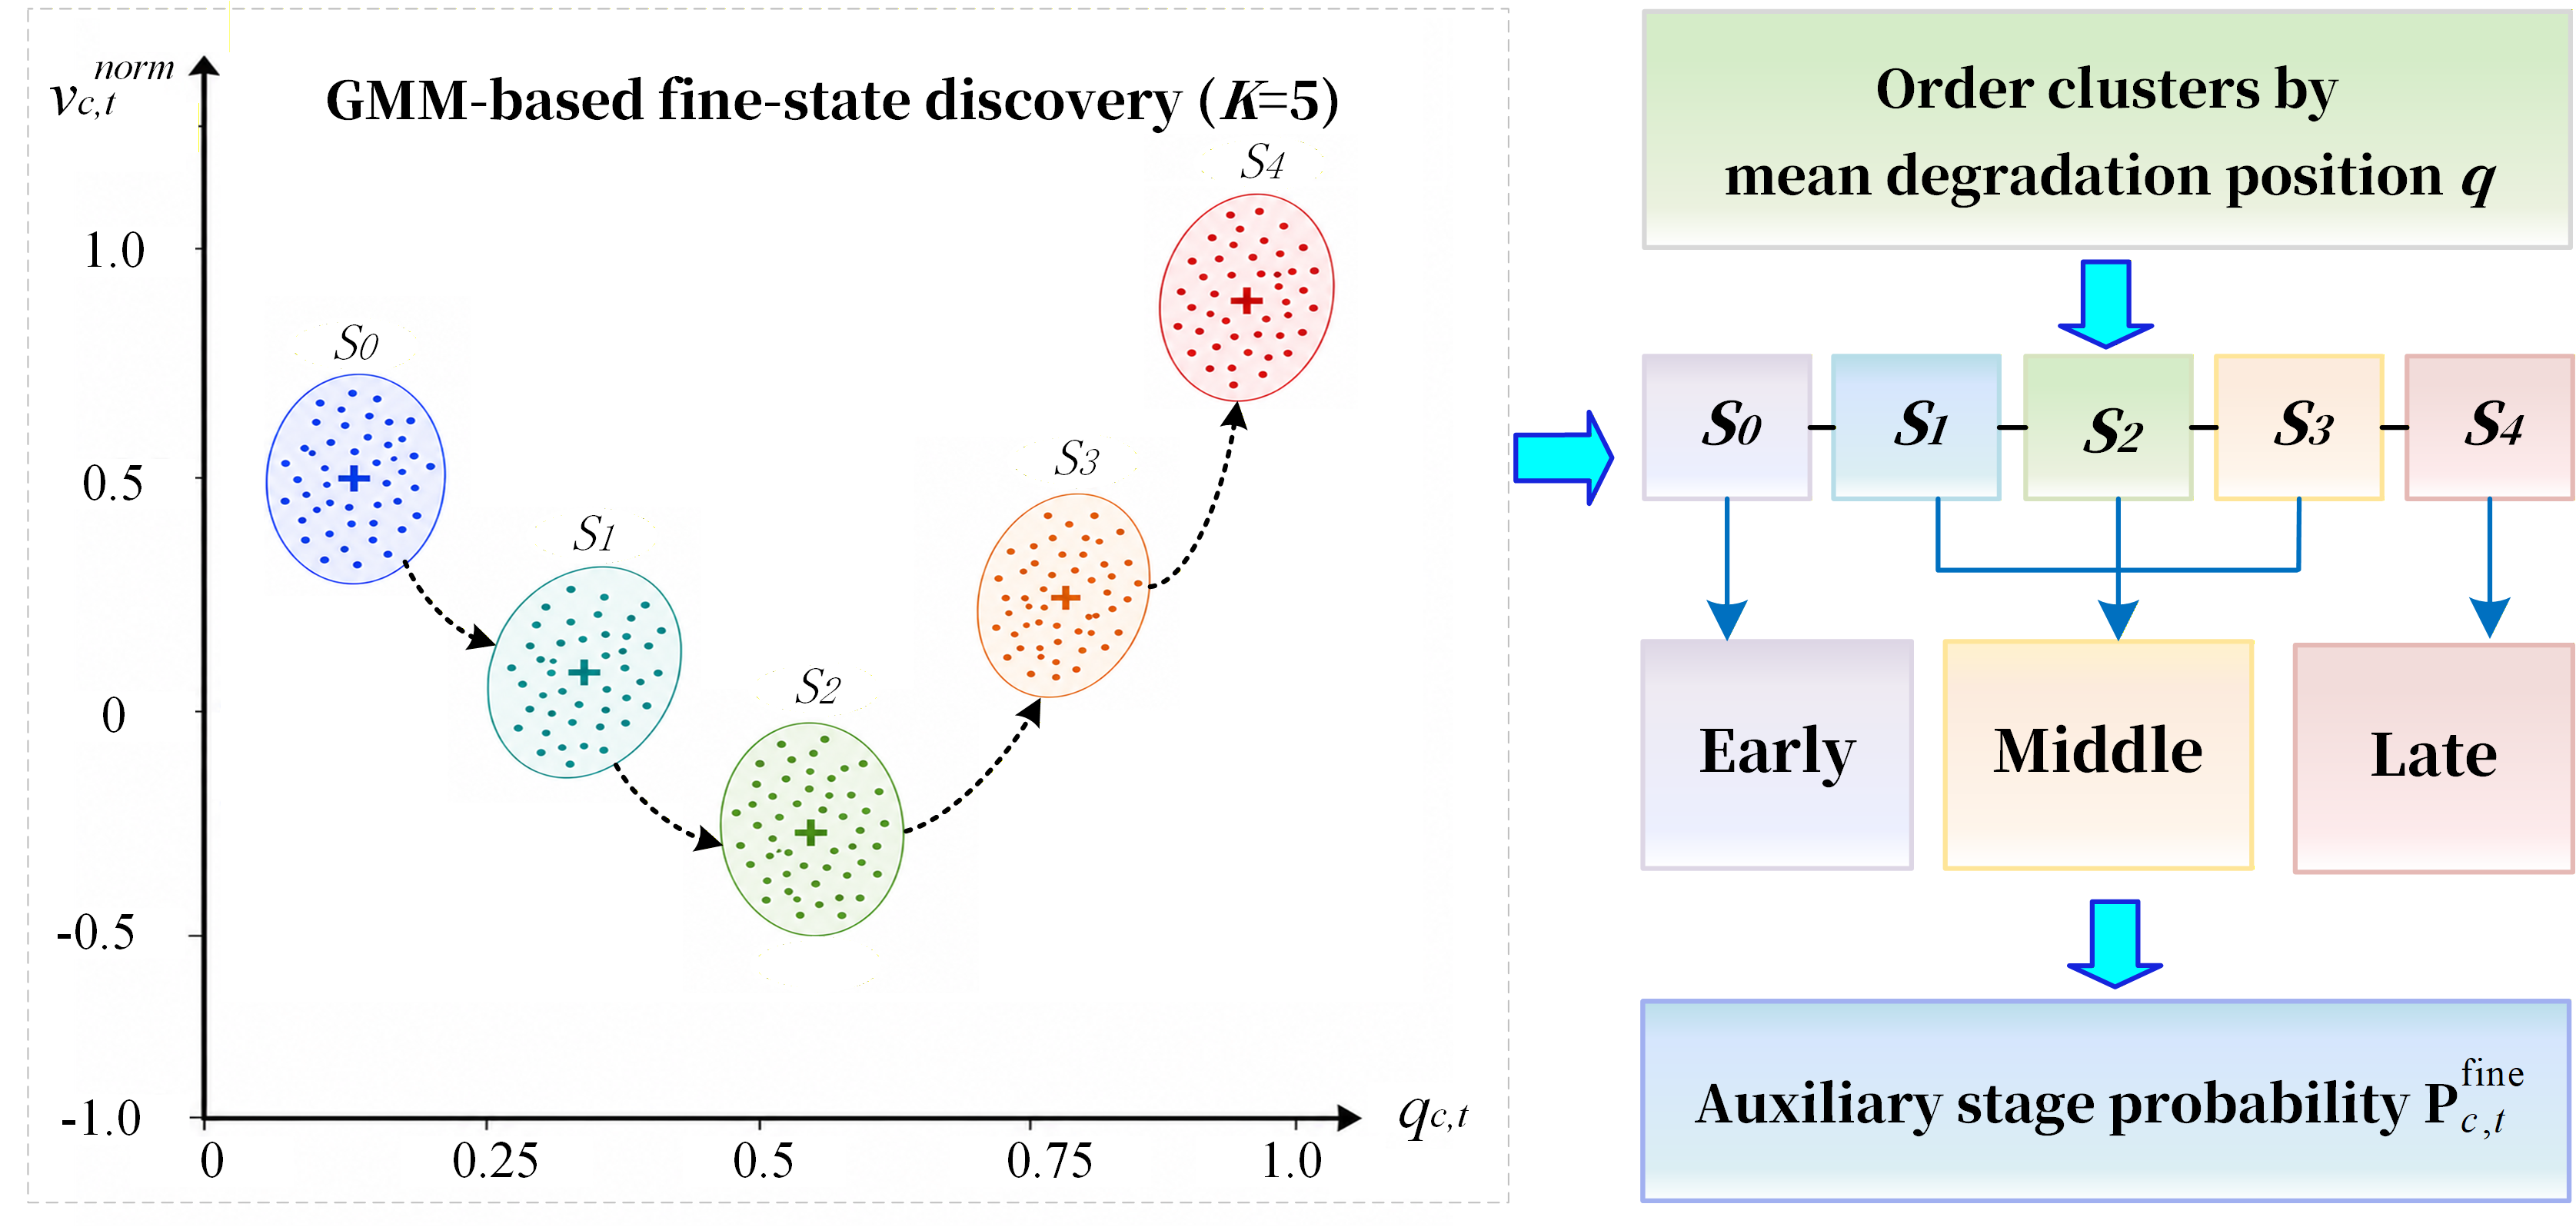
\includegraphics[width=0.68\textwidth,keepaspectratio]{figures/fig3.png}
    \caption{Fine-grained state construction and stage mapping.}
    \label{fig:3}
  \end{figure}
\subsection{Multi-Task Temporal Modeling and Ordered Probabilistic Inference}
\label{sec:ordered_inference}
  After the procedures in \secsref{sec:stage_semantics}{sec:fine_state}, each cutting sample is assigned a macro-stage label $s_{c,t}$, a fine-grained degradation state $g_{c,t}$, and a relative degradation position $q_{c,t}$. A multi-task temporal network is then built to learn a shared degradation representation from these supervisory signals, and ordered probabilistic inference is used to convert instantaneous stage predictions into life-cycle-consistent stage probabilities.

  Let $\mathbf{x}_{c,t}\in \mathbb{R}^{d}$ denote the condition-relative feature vector of the $t$-th cut under condition $c$. A sliding window of length $L$ is used to form the temporal input:
  \begin{equation}
    \begin{aligned}
      \mathbf{X}_{c,t}=[\mathbf{x}_{c,t-L+1},\mathbf{x}_{c,t-L+2},\ldots,\mathbf{x}_{c,t}]\in \mathbb{R}^{L\times d}
    \end{aligned}
  \end{equation}
  
  Tool wear stage is a temporal degradation state rather than an isolated sample attribute. \citet{ref21} showed that local variation patterns and cross-time dependencies are important for RUL prediction based on multi-scale time--frequency milling force information. Accordingly, a TCN-GRU backbone is adopted, where TCN captures local degradation patterns and GRU models stage-evolution dependencies:
  \begin{equation}
    \begin{aligned}
      \mathbf{H}_{c,t}^{\mathrm{TCN}}=f_{\mathrm{TCN}}(\mathbf{X}_{c,t}),\\
      \mathbf{h}_{c,t}=f_{\mathrm{GRU}}(\mathbf{H}_{c,t}^{\mathrm{TCN}})
    \end{aligned}
  \end{equation}
  where $\mathbf{h}_{c,t}$ is the shared degradation representation. 
  
  Three output heads are built on $\mathbf{h}_{c,t}$: a macro-stage classification head, a fine-grained state classification head, and a degradation-position regression head. They are respectively defined as
\begin{equation}
	\begin{aligned}
		\mathbf{p}_{c,t}^{\mathrm{raw}}
		&=
		\operatorname{Softmax}(\mathbf{W}_{s}\mathbf{h}_{c,t}+\mathbf{b}_{s}),\\
		\mathbf{p}_{c,t}^{\mathrm{raw}}
		&=
		[p_{c,t}^{\mathrm{raw},E},p_{c,t}^{\mathrm{raw},M},p_{c,t}^{\mathrm{raw},L}],\\
		\mathbf{p}_{c,t}^{g}
		&=
		\operatorname{Softmax}(\mathbf{W}_{g}\mathbf{h}_{c,t}+\mathbf{b}_{g}),\\
		\hat{q}_{c,t}
		&=
		\sigma(\mathbf{W}_{q}\mathbf{h}_{c,t}+b_q).
	\end{aligned}
	\label{eq:multi_task_outputs}
\end{equation}
  where $\sigma(\cdot)$ denotes the sigmoid activation function, $\mathbf{p}_{c,t}^{\mathrm{raw}}$ denotes the raw early--middle--late probability, $\mathbf{p}_{c,t}^{g}$ corresponds to the ordered fine-grained states $S_{0},\ldots,S_{4}$, and $\hat{q}_{c,t}\in [0,1]$ is the estimated relative degradation position.

  The overall training objective is
  \begin{equation}
    \begin{aligned}
      L=\lambda_{s}L_{\mathrm{stage}}+\lambda_{g}L_{\mathrm{fine}}+\lambda_{q}L_q+\lambda_{m}L_{\mathrm{mono}}
    \end{aligned}
  \end{equation}
  where $L_{\mathrm{stage}}$ and $L_{\mathrm{fine}}$ are cross-entropy losses for macro-stage and fine-grained state classification, $L_q$ is the Smooth L1 loss for degradation-position regression, and $L_{\mathrm{mono}}$ is a weak monotonic regularization term.

  Although $\mathbf{p}_{c,t}^{\mathrm{raw}}$ provides sensing-based instantaneous discrimination, it may be affected by noise, local disturbances, and cross-condition shifts. Therefore, a degradation-position prior is constructed from $\hat{q}_{c,t}$. Let $c_{E}$, $c_{M}$, and $c_{L}$ denote the position centers of the early, middle, and late stages. The basic prior is
  \begin{equation}
    \begin{aligned}
      \phi_k(\hat{q}_{c,t})
      =
      \exp\left[
      -\frac{(\hat{q}_{c,t}-c_k)^2}{2\sigma^2}
      \right],\quad k\in\{E,M,L\}
    \end{aligned}
  \end{equation}
  
  To reduce two-sided compression of the middle stage, premature-early inhibition and late suppression are introduced as
  \begin{equation}
 	\begin{aligned}
 		g_E(\hat{q}_{c,t})
 		&=
 		\sigma\!\left[\kappa_E(\tau_E-\hat{q}_{c,t})\right],\\
 		\phi_E'(\hat{q}_{c,t})
 		&=
 		\phi_E(\hat{q}_{c,t})g_E(\hat{q}_{c,t}),\\
 		g_L(\hat{q}_{c,t})
 		&=
 		\sigma\!\left[\kappa_L(\hat{q}_{c,t}-\tau_L)\right],\\
 		\phi_L'(\hat{q}_{c,t})
 		&=
 		\phi_L(\hat{q}_{c,t})g_L(\hat{q}_{c,t}).
 	\end{aligned}
 	\label{eq:dual_side_inhibition}
   \end{equation}
  Here, $g_{E}(\cdot )$ suppresses persistently high early probabilities after the early region, whereas $g_{L}(\cdot )$ suppresses premature assignment to the late stage. To avoid over-compression of the middle stage, a middle-floor prior is imposed:
  \begin{equation}
    \begin{aligned}
      \phi_{M}^{'}(\hat{q}_{c,t})=\max(\phi_{M}(\hat{q}_{c,t}),p_{\min})
    \end{aligned}
  \end{equation}
  
  The adjusted priors are normalized as
  \begin{equation}
    \begin{aligned}
      \mathbf{p}_{c,t}^{\mathrm{prior}}
      =
      \operatorname{Normalize}\!\left[
      \phi_{E}^{'}(\hat{q}_{c,t}),
      \phi_{M}^{'}(\hat{q}_{c,t}),
      \phi_{L}^{'}(\hat{q}_{c,t})
      \right]
    \end{aligned}
  \end{equation}
  
  The final probability integrates raw stage discrimination, fine-state auxiliary information, and degradation-position constraints. First, the auxiliary probability is computed by
  \begin{equation}
    \begin{aligned}
      \mathbf{p}_{c,t}^{\mathrm{aux}}=\omega_{f}\mathbf{p}_{c,t}^{\mathrm{fine}}+(1-\omega_{f})\mathbf{p}_{c,t}^{\mathrm{prior}}
    \end{aligned}
  \end{equation}
  and then fused with the raw stage probability:
  \begin{equation}
    \begin{aligned}
      \mathbf{p}_{c,t}^{\mathrm{mix}}=\eta\mathbf{p}_{c,t}^{\mathrm{raw}}+(1-\eta)\mathbf{p}_{c,t}^{\mathrm{aux}}
    \end{aligned}
  \end{equation}
  where $\omega_{f}$ and $\eta$ are fusion weights. This yields a mixed probability that combines sensing-based discrimination, fine-grained degradation structure, and position-aware constraints.

  Since tool wear generally follows the ordered progression from early to middle and late, causal ordered filtering is further used to suppress reverse transitions and non-physical probability fluctuations. The stage transition matrix is defined as
  \begin{equation}
	\mathbf{A}=
	\begin{bmatrix}
		0.9400 & 0.0550 & 0.0050\\
		0.0050 & 0.9550 & 0.0400\\
		0.0005 & 0.0100 & 0.9895
	\end{bmatrix}
	\label{eq:transition_matrix}
  \end{equation}
  
  For the $t$-th cut, the ordered stage probability is recursively updated by
  \begin{equation}
    \boldsymbol{\alpha}_{c,t}
    =
    \frac{
    (\boldsymbol{\alpha}_{c,t-1}\mathbf{A})\odot \mathbf{p}_{c,t}^{\mathrm{mix}}
    }{
    \sum [(\boldsymbol{\alpha}_{c,t-1}\mathbf{A})\odot \mathbf{p}_{c,t}^{\mathrm{mix}}]
    }
    \label{eq:ordered_filter}
  \end{equation}
  where $\odot$ denotes element-wise multiplication. To balance temporal smoothness and boundary responsiveness, the mixed and ordered probabilities are finally combined as
  \begin{equation}
    \mathbf{p}_{c,t}^{\mathrm{final}}
    =
    (1-\beta)\mathbf{p}_{c,t}^{\mathrm{mix}}
    +
    \beta\boldsymbol{\alpha}_{c,t}
    \label{eq:final_probability}
  \end{equation}
  where $\beta$ is the fusion weight of the ordered probability.

  The final probabilistic stage representation is
  \begin{equation}
    \begin{aligned}
      \mathbf{p}_{c,t}^{\mathrm{final}}=[p_{c,t}^{\mathrm{final},E},p_{c,t}^{\mathrm{final},M},p_{c,t}^{\mathrm{final},L}]
    \end{aligned}
  \end{equation}
  
  Overall, \figref{fig:4} summarizes the multi-task degradation representation and ordered stage inference process.

  \begin{figure}[pos=!htbp]
    \centering
    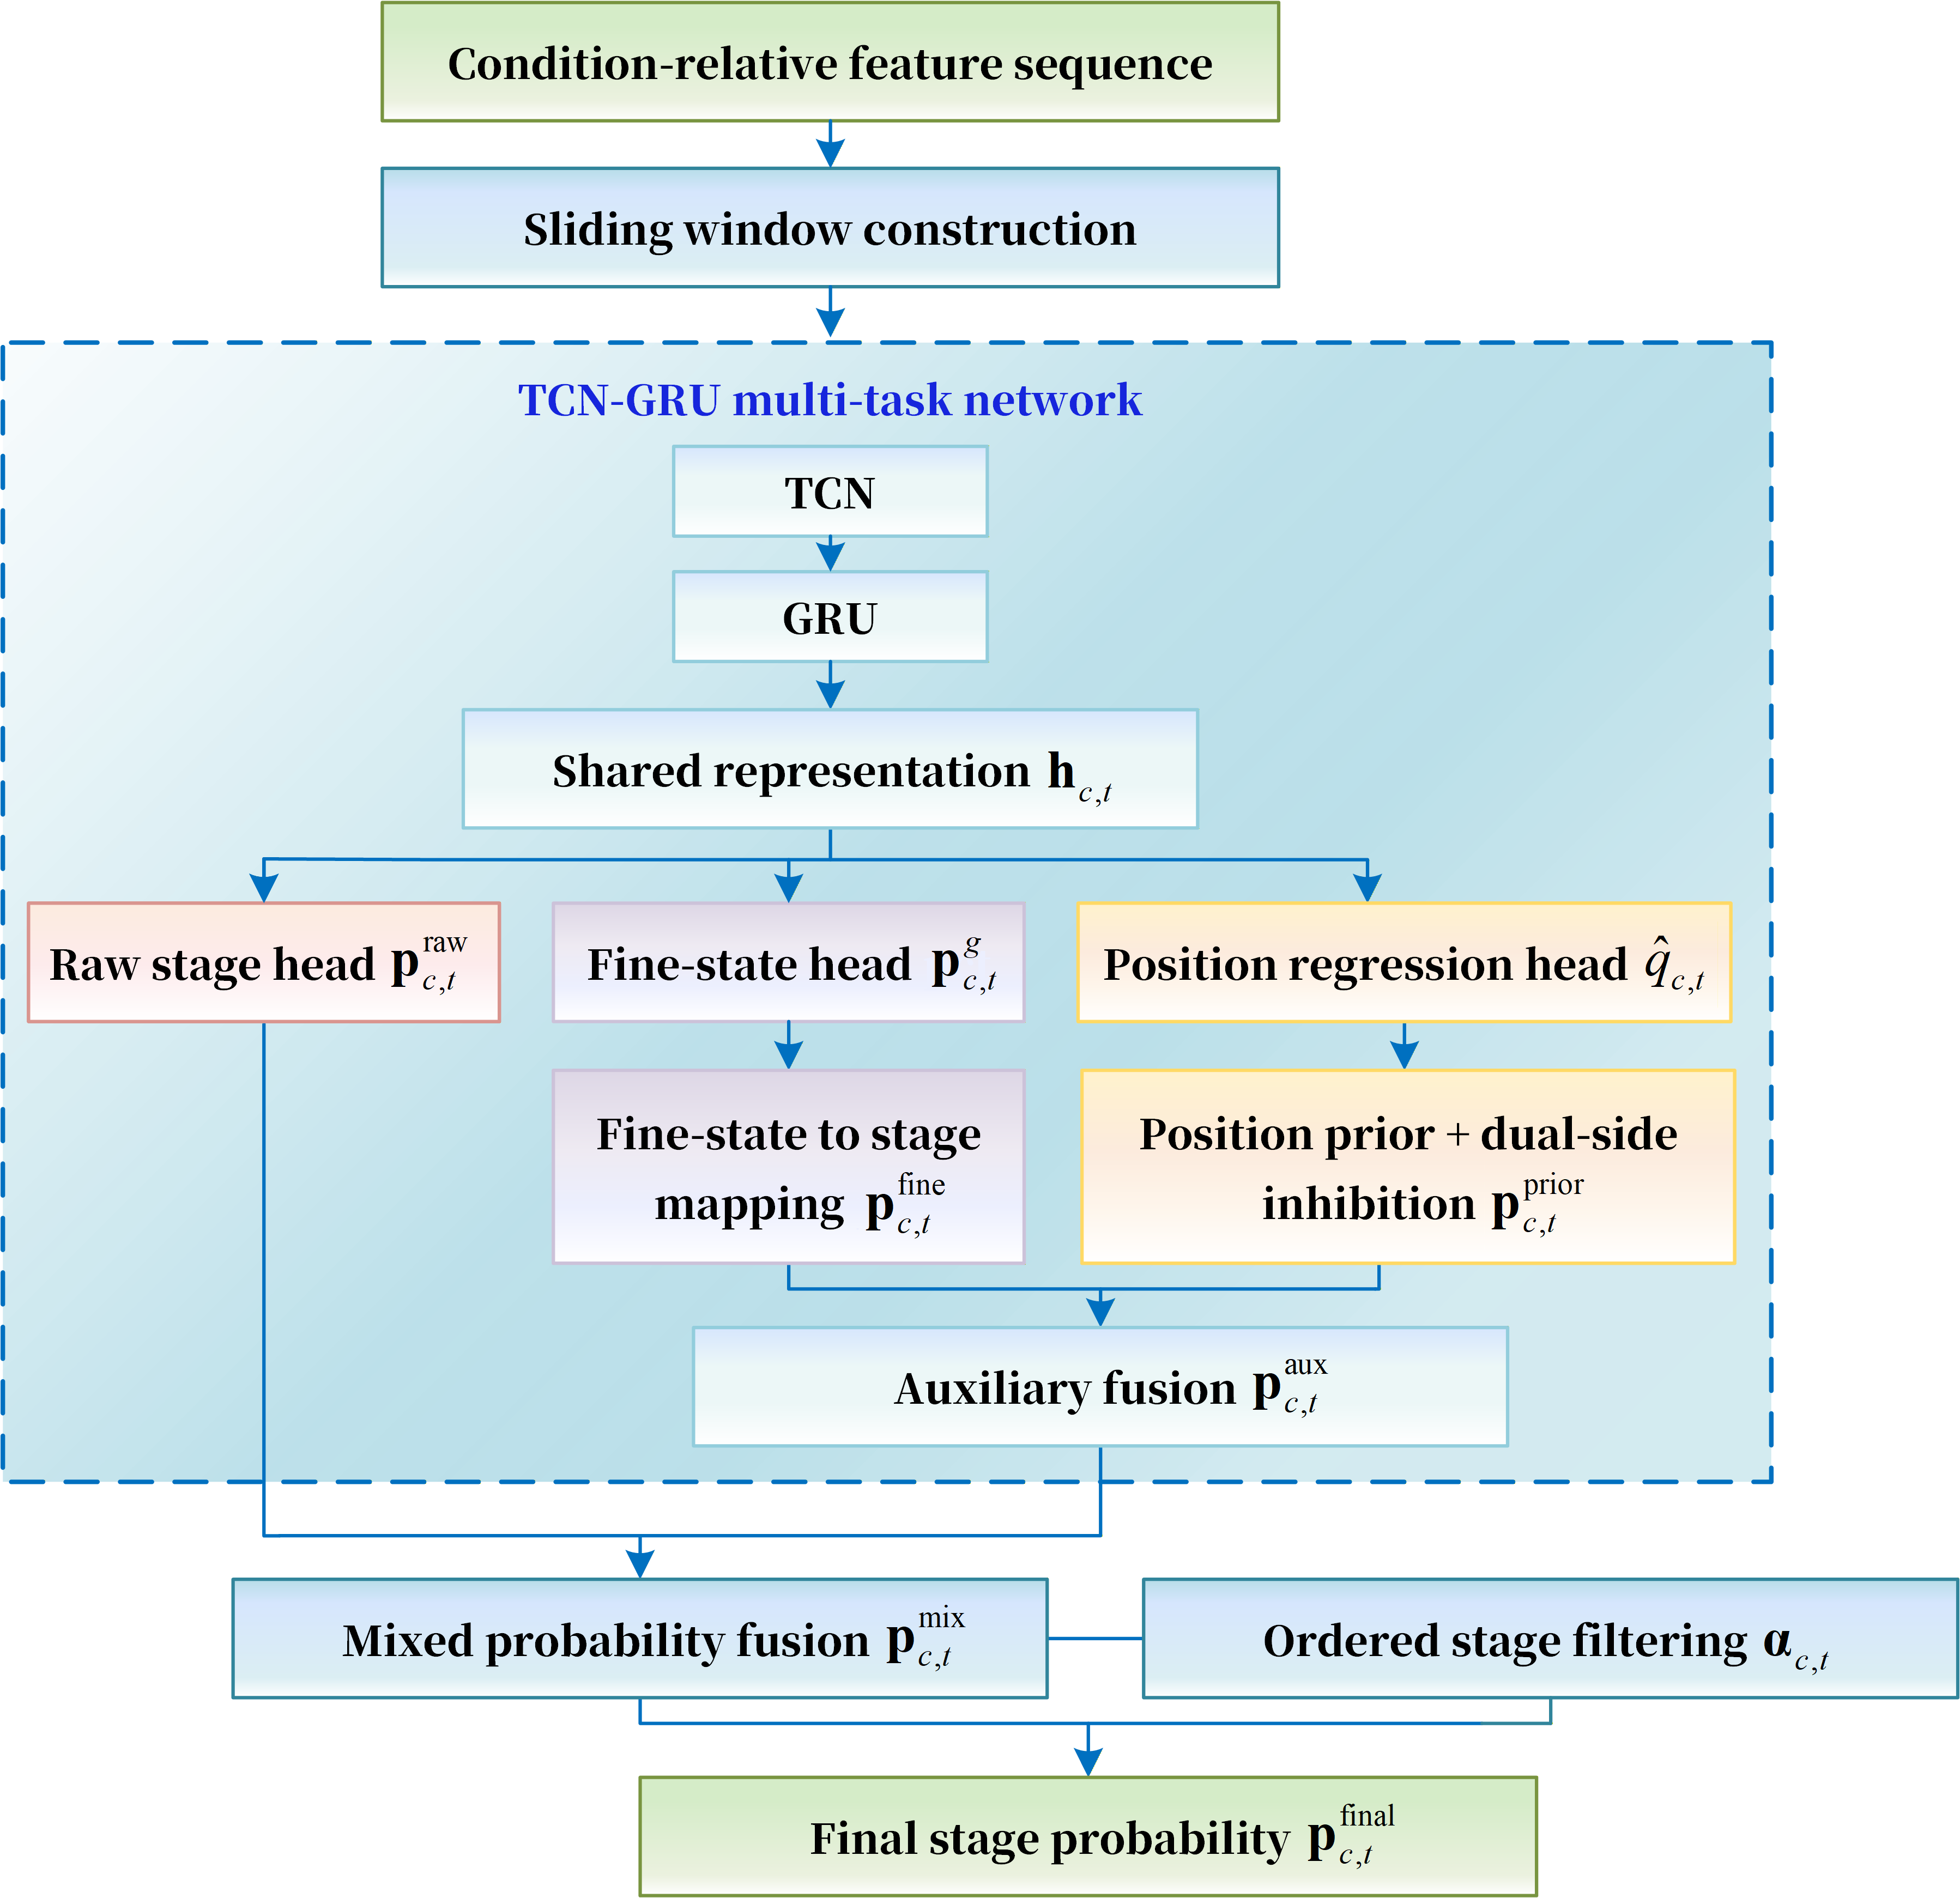
\includegraphics[width=0.68\textwidth,keepaspectratio]{figures/fig4.png}
    \caption{Multi-task degradation representation and ordered stage inference.}
    \label{fig:4}
  \end{figure}
\subsection{Algorithm Procedure}
\label{sec:algorithm}
  The overall implementation of DC-PSR is divided into two stages: offline training and online monitoring. In the offline stage, relative stage semantics are constructed, fine-grained degradation states are mined, and the multi-task temporal network is trained. In the online stage, the probabilistic stage representation is generated using the current and historical monitoring information. The detailed procedure is summarized in Algorithm 1.

  \begin{algorithm}[htbp]
    \caption{DC-PSR for Cross-Condition Tool Wear Monitoring}
    \label{alg:dcpsr}
    \begin{algorithmic}[1]
      \Require Training data $D_{tr}=\{x_{c,t},VB_{c,t}\}$; window length $L$; fine-state number $K$; fusion weights $\eta,\omega_{f},\beta$.
      \Ensure Final stage probability $\mathbf{p}_{c,t}^{\mathrm{final}}$, predicted stage $s_{c,t}$, and degradation position $\hat{q}_{c,t}$.
      \Statex \textbf{{Part 1. Offline training and prior construction}}
      \For{each training condition $c\in C_{tr}$}
      \State Smooth $VB_{c,t}$ and compute $q_{c,t}$ and $\nu_{c,t}^{\mathrm{norm}}$.
      \State Define $s_{c,t}\in \{E,M,L\}$ using $Q_{E}$, $Q_{L}$, and $Q_{\nu}$.
      \EndFor
      \State Select sensitive and condition-invariant features using the multi-objective score $Score_{j}$.
      \State Fit a $K$-component GMM on $u_{c,t}=[q_{c,t},\nu_{c,t}^{\mathrm{norm}}]^{T}$.
      \State Map ordered fine-grained states $g_{c,t}\in \{S_{0},\ldots,S_{K-1}\}$ to macro stages.
      \State Train the TCN-GRU network by minimizing $L=\lambda_{s}L_{\mathrm{stage}}+\lambda_{g}L_{\mathrm{fine}}+\lambda_{q}L_q+\lambda_{m}L_{\mathrm{mono}}$.
      \Statex \textbf{{Part 2. Online monitoring and ordered probabilistic inference}}
      \For{each time step $t$ in the test condition $c\in C_{te}$}
      \State Generate online features $\left\{x^{rel}\right\}$ and construct sliding-window $\mathbf{X}_{c,t}$.
      \State Infer $\mathbf{p}_{c,t}^{\mathrm{raw}}$, $\mathbf{p}_{c,t}^{g}$, and $\hat{q}_{c,t}$ via parallel output heads.
      \State Map $\mathbf{p}_{c,t}^{g}$ to $\mathbf{p}_{c,t}^{\mathrm{fine}}$, and construct $\mathbf{p}_{c,t}^{\mathrm{prior}}$ from $\hat{q}_{c,t}$ with dual-side inhibition.
      \State Fuse raw probability, fine-state probability and position prior to obtain $\mathbf{p}_{c,t}^{\mathrm{mix}}$.
      \State Apply causal ordered filtering with $\mathbf{A}$, and generate $\mathbf{p}_{c,t}^{\mathrm{final}}=\left(1-\beta\right)\mathbf{p}_{c,t}^{\mathrm{mix}}+\beta\boldsymbol{\alpha}_{c,t}$
      \State Assign the predicted stage $s_{c,t}=\arg\max_{s\in \{E,M,L\}}p_{c,t}^{\mathrm{final},s}$.
      \EndFor
    \end{algorithmic}
  \end{algorithm}
  \section{Experimental Settings}
\label{sec:experiments}
  \subsection{Datasets}
\label{sec:datasets}
  Two public milling datasets, \href{https://www.kaggle.com/datasets/rabahba/phm-data-challenge-2010}{PHM2010} and \href{https://www.nasa.gov/intelligent-systems-division/discovery-and-systems-health/pcoe/pcoe-data-set-repository/}{NASA Milling}, are used for validation. PHM2010 provides multi-source sensing signals and flank wear measurements under several milling conditions and serves as the main benchmark for cross-condition evaluation. NASA Milling contains more cutting cases but fewer samples per case, and is used as an external validation dataset under small-sample, multi-case settings.

  After feature extraction from raw signals, all data are organized as run-level feature sequences. \citet{ref35} also showed that milling sensing features can effectively support tool wear state recognition. \figref{fig:5} shows the PHM2010 high-speed milling platform.
  \begin{figure}[pos=!htbp]
	\centering
	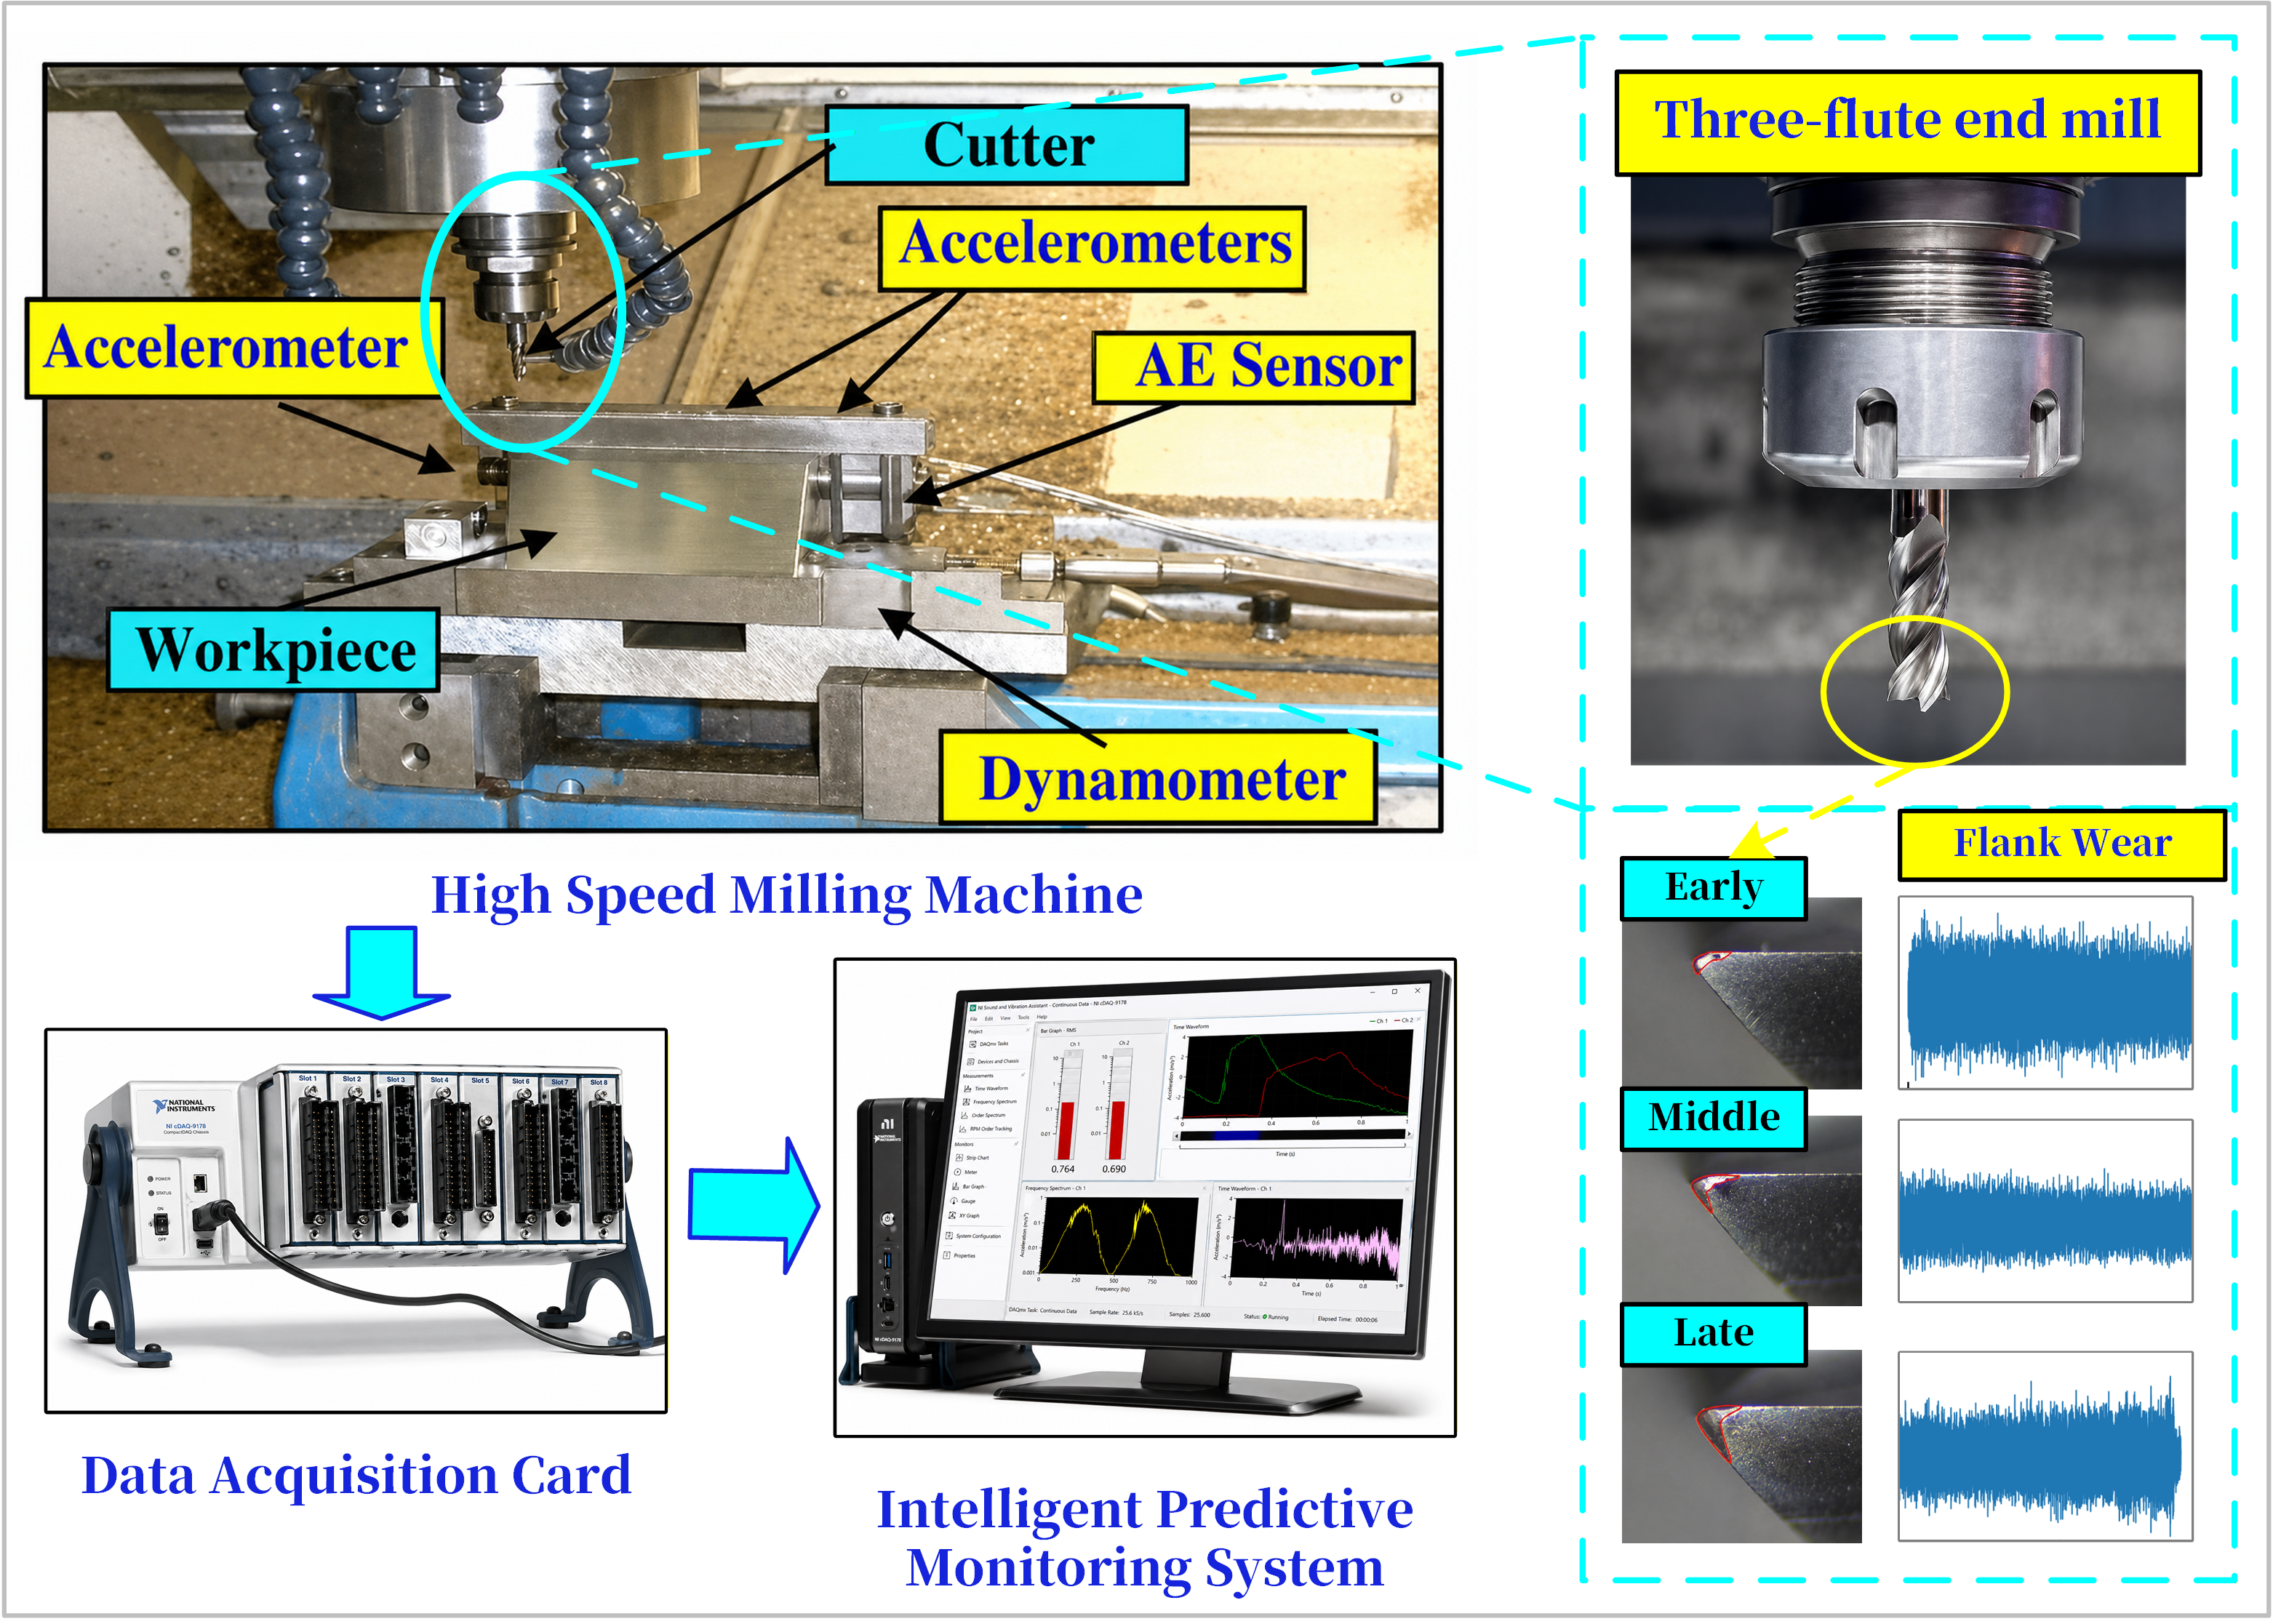
\includegraphics[width=0.8\textwidth,keepaspectratio]{figures/fig5.png}
	\caption{PHM2010 tool wear experimental platform.}
	\label{fig:5}
 \end{figure}

To further examine the link between stage state and the reliability of continuous degradation representation, the wear-estimation errors of aligned window samples in the external test condition are analyzed, as shown in Table~\ref{tab:stage_bias}. Here, Bias is defined as $\mathrm{mean}(\widehat{VB}-VB)$, where negative and positive values indicate underestimation and overestimation, respectively. The results reveal clear stage-related bias: the early stage is systematically underestimated, the late stage is systematically overestimated, and the middle stage shows relatively smaller errors. This indicates that stage state is not merely a discrete class label, but also reflects the reliability variation of degradation representation across different life-cycle regions. Therefore, a continuous, ordered, and degradation-consistent probabilistic stage state is necessary.

\begin{table}[!htbp]
	\centering
	\scriptsize
	\caption{Stage-related bias in wear-value estimation.}
	\label{tab:stage_bias}
	\begin{adjustbox}{max width=\textwidth}
		\begin{tabular}{lccccc}
			\toprule
			\textbf{True stage} & \textbf{Samples} & \textbf{MAE} & \textbf{RMSE} & \textbf{Bias} & \textbf{MaxAE} \\
			\midrule
			early  & 106 & 12.21 & 12.52 & -12.21 & 16.78 \\
			middle & 97  & 4.52  & 5.68  & -2.75  & 11.26 \\
			late   & 93  & 12.35 & 13.21 & 12.34  & 20.63 \\
			\bottomrule
		\end{tabular}
	\end{adjustbox}
\end{table}
  \figref{fig:6} shows the time- and frequency-domain characteristics of milling force signals at different wear stages. For the test condition, $q_{c,t}$ and the stage labels derived from the complete VB sequence are used only as offline evaluation references.

  \begin{figure}[pos=!htbp]
    \centering
    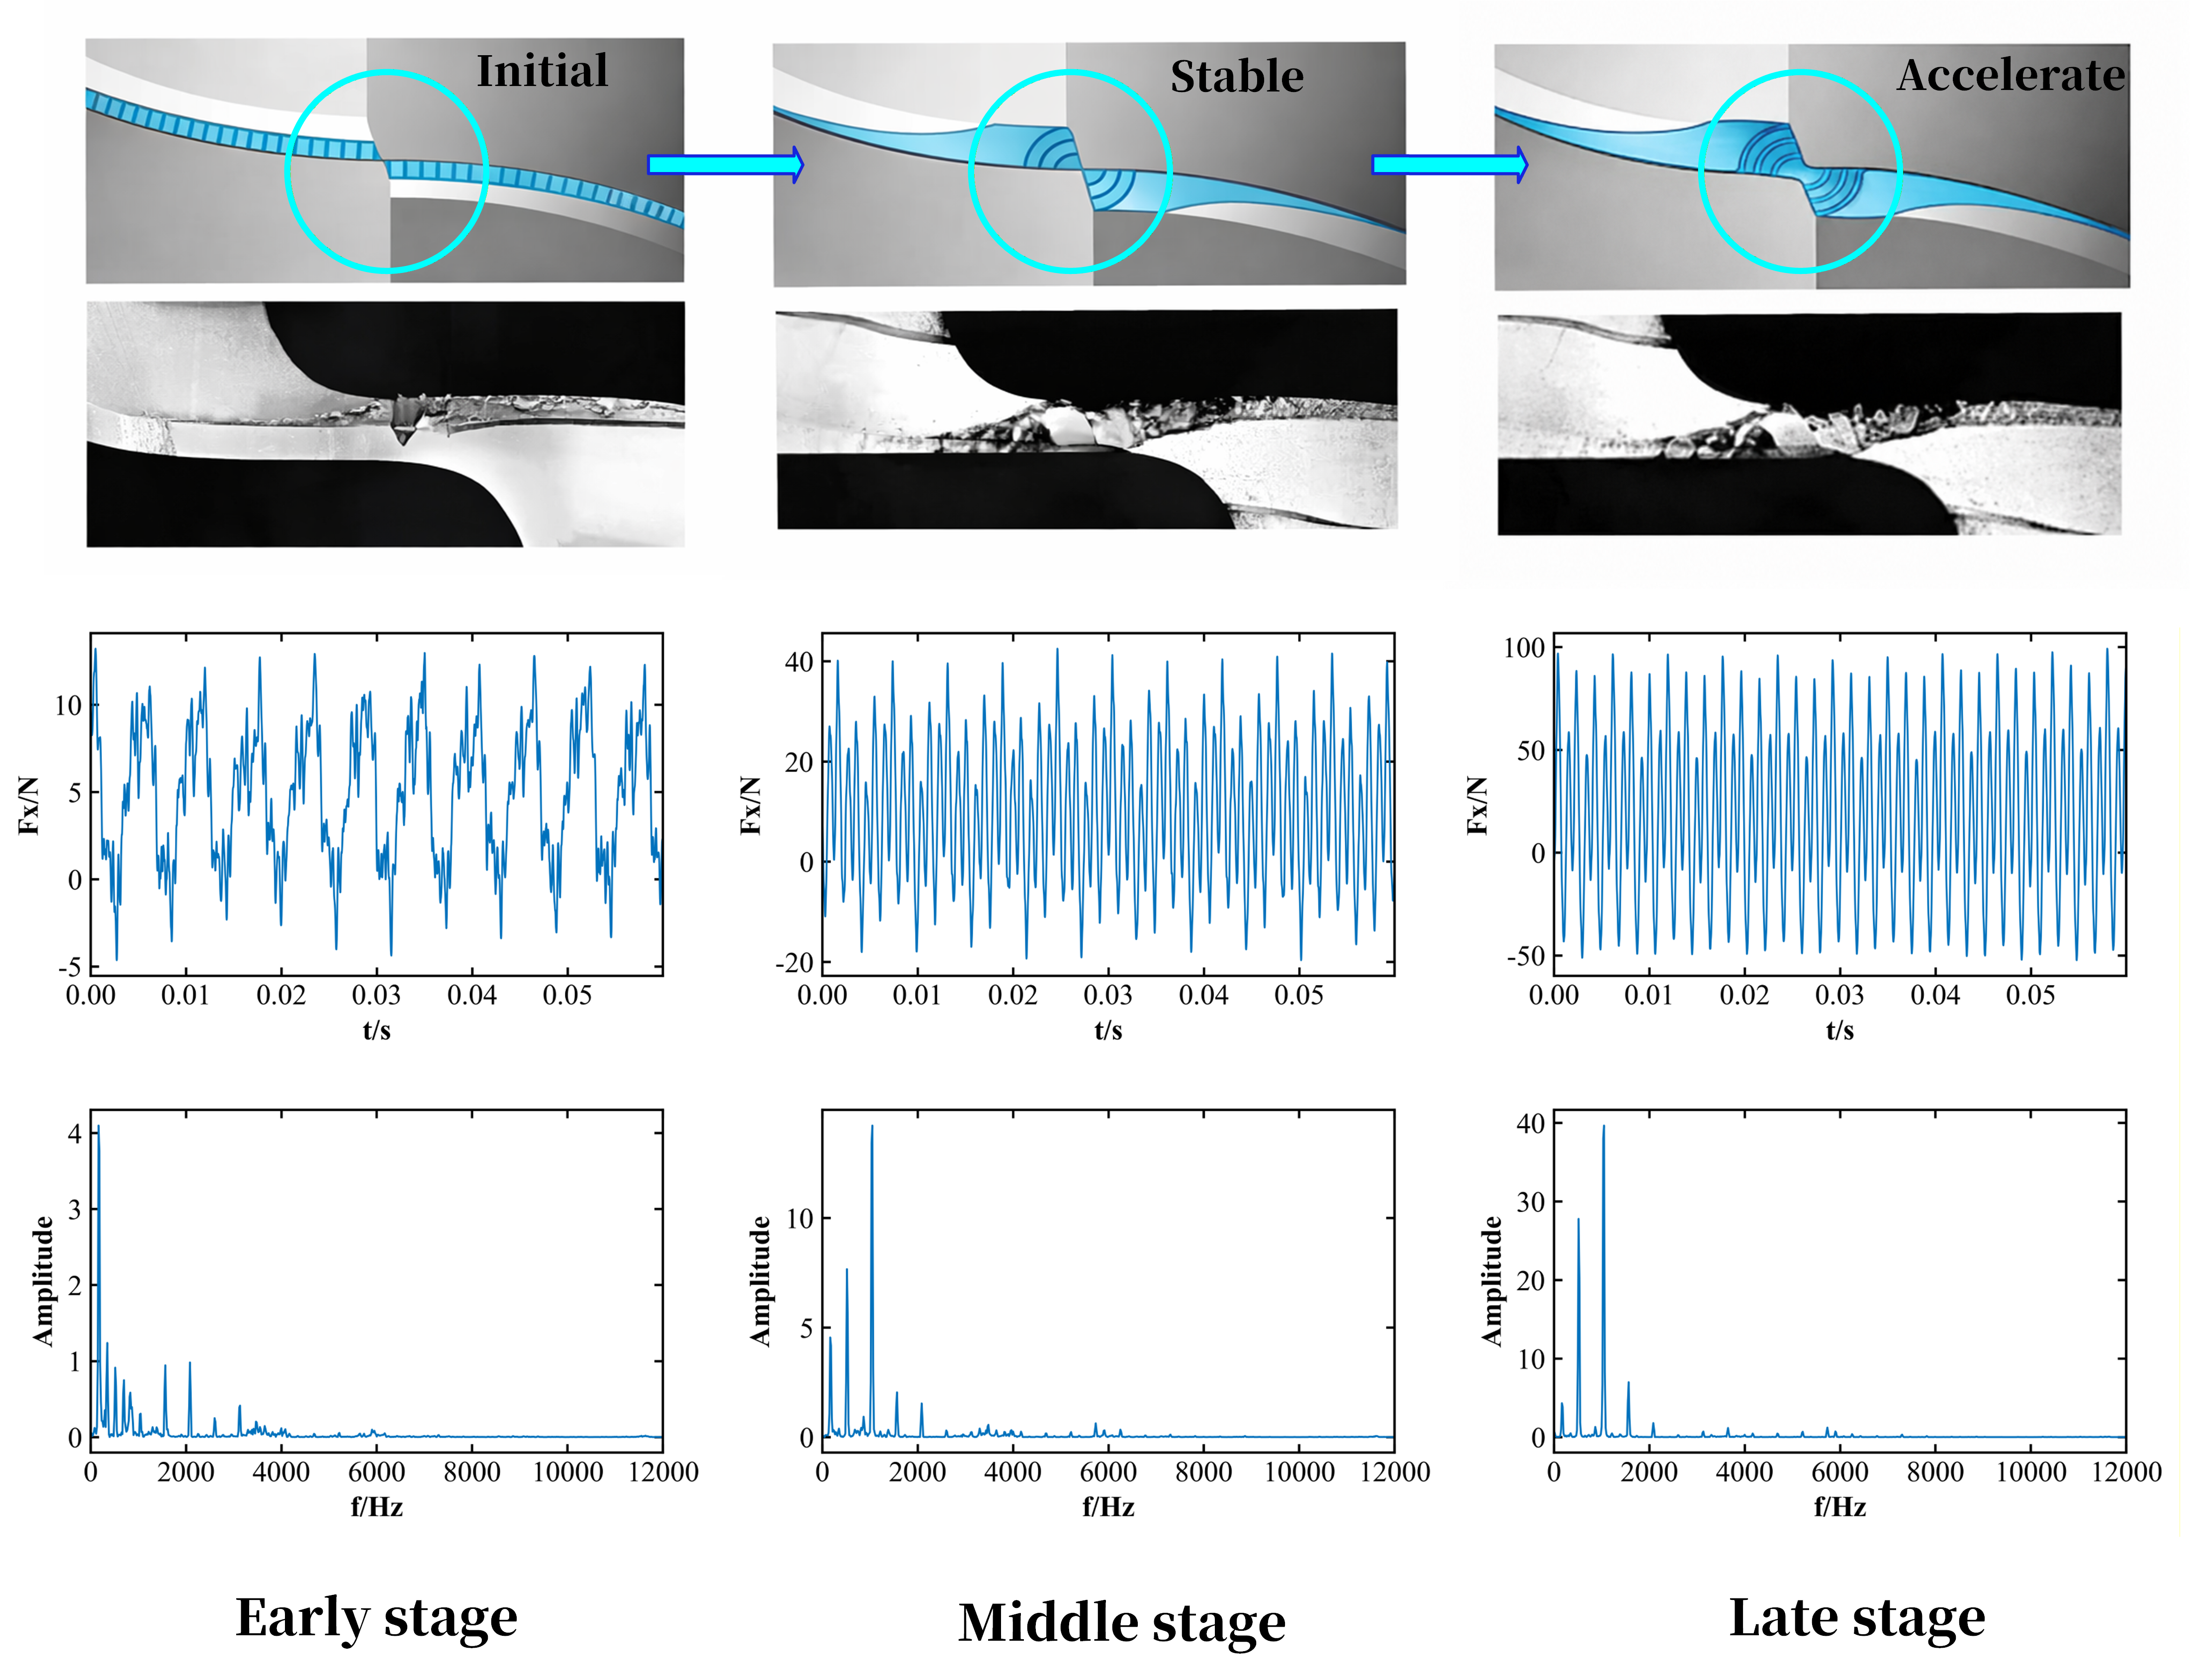
\includegraphics[width=0.8\textwidth,keepaspectratio]{figures/fig6.png}
    \caption{Milling force signals at different wear stages.}
    \label{fig:6}
  \end{figure}
\subsection{Experimental Design}
  Three experiments are conducted to evaluate DC-PSR: main comparison, cross-condition generalization, and ablation analysis. They assess the overall stage representation capability, generalization stability under different transfer settings, and the contribution of each module, respectively. The main comparison is performed on the C1+C4 $\to$C6 task, with the compared methods listed in \tabref{tab:3}.

  \begin{table}[!htbp]
    \centering
    \scriptsize
  \caption{Baseline methods.}
    \label{tab:3}
    \begin{adjustbox}{max width=\textwidth}
      \begin{tabular}{llll}
        \toprule
        \textbf{ID} & \textbf{Method} & \textbf{Stage definition} & \textbf{Model} \\
        \midrule
        B1 & Fixed-stage Rule & Fixed threshold & Rule \\
        B2 & Relative-stage Rule & Condition-relative stage & Rule \\
        B3 & Fixed-stage RF & Fixed threshold & RF \\
        B4 & Relative-stage SVM & Condition-relative stage & SVM \\
        B5 & Relative-stage RF & Condition-relative stage & RF \\
        B6 & Relative-stage XGBoost & Condition-relative stage & XGBoost \\
        B7 & Relative-stage MLP & Condition-relative stage & MLP \\
        B8 & Relative-stage TCN & Condition-relative stage & TCN \\
        B9 & Relative-stage GRU & Condition-relative stage & GRU \\
        B10 & Relative-stage TCN-GRU & Condition-relative stage & TCN-GRU \\
        B11 & Multi-task TCN-GRU & Condition-relative stage & TCN-GRU + auxiliary heads \\
        B12 & DC-PSR & Condition-relative stage & Proposed \\
        \bottomrule
      \end{tabular}
    \end{adjustbox}
  \end{table}
  The baselines are designed with reference to recent studies on deep temporal modeling for small-sample tool wear prediction \citep{ref37,ref44}. B1--B3 examine fixed-threshold stage definitions; B4--B6 are conventional machine-learning classifiers; B7--B10 are deep temporal baselines; B11 is the multi-task TCN-GRU baseline; and B12 is the complete DC-PSR.

  Since heterogeneous working conditions can affect degradation representation and RUL prediction stability \citep{ref33}, additional cross-condition tasks are constructed on PHM2010 and NASA Milling, as shown in \tabref{tab:4}. PHM2010 is used for dual-source and single-source transfer tasks, whereas NASA Milling provides external cross-case validation under small-sample and more heterogeneous cutting conditions.

  \begin{table}[!htbp]
    \centering
    \scriptsize
  \caption{Cross-condition generalization tasks.}
    \label{tab:4}
    \begin{adjustbox}{max width=\textwidth}
      \begin{tabular}{llll}
        \toprule
        \textbf{Dataset} & \textbf{Task} & \textbf{Training conditions} & \textbf{Test conditions} \\
        \midrule
        PHM2010 & D1 & C1 + C4 & C6 \\
        & D2 & C4 + C6 & C1 \\
        & S1 & C4 & C1 \\
        & S2 & C6 & C1 \\
        NASA Milling & N1 & 1, 2, 4, 5, 6, 7, 8, 9, 10, 11, 13, 14 & 3, 12, 15, 16 \\
        & N2 & 1, 3, 4, 5, 6, 7, 11, 12, 13, 14, 15, 16 & 2, 8, 9, 10 \\
        & N3 & 1, 2, 4, 6, 7, 8, 9, 11, 13, 14, 15, 16 & 3, 5, 10, 12 \\
        & N4 & 1, 2, 3, 4, 5, 6, 7, 9, 10, 11, 14, 15 & 8, 12, 13, 16 \\
        \bottomrule
      \end{tabular}
    \end{adjustbox}
  \end{table}
  The ablation study uses the same data split, feature input, and backbone network. Fine-grained state assistance, degradation-position prior, ordered filtering, and final fusion are progressively introduced to quantify their effects. The settings are listed in \tabref{tab:5}.

  \begin{table}[!htbp]
    \centering
    \scriptsize
  \caption{Ablation settings.}
    \label{tab:5}
    \begin{adjustbox}{max width=\textwidth}
      \begin{tabular}{llll}
        \toprule
        \textbf{ID} & \textbf{Method} & \textbf{Information used} & \textbf{Output} \\
        \midrule
        A1 & Raw & Stage head & $\mathbf{p}_{c,t}^{\mathrm{raw}}$ \\
        A2 & Raw + Fine & Stage head + Fine-state head & $\mathbf{p}_{c,t}^{\mathrm{raw}}$ + $\mathbf{p}_{c,t}^{\mathrm{fine}}$ \\
        A3 & Raw + Prior & Stage head + $q$-prior & $\mathbf{p}_{c,t}^{\mathrm{raw}}$ + $\mathbf{p}_{c,t}^{\mathrm{prior}}$ \\
        A4 & Mix & Stage head + Fine-state head + $q$-prior & $\mathbf{p}_{c,t}^{\mathrm{mix}}$ \\
        A5 & Ordered & Mix + ordered filtering & $\boldsymbol{\alpha}_{c,t}$ \\
        A6 & Final & All & $\mathbf{p}_{c,t}^{\mathrm{final}}$ \\
        \bottomrule
      \end{tabular}
    \end{adjustbox}
  \end{table}
  \subsection{Parameter and Evaluation Metrics}
\label{sec:metrics}
  DC-PSR contains network parameters and probability-fusion parameters. Network parameters are selected through bidirectional proxy validation between training conditions, while fusion parameters are determined using the internal validation set. The final settings are given in \tabref{tab:6}.

  \begin{table}[!htbp]
    \centering
    \scriptsize
  \caption{Model parameters.}
    \label{tab:6}
    \begin{adjustbox}{max width=\textwidth}
      \begin{tabular}{llll}
        \toprule
        \textbf{Category} & \textbf{Parameter} & \textbf{Description} & \textbf{Value} \\
        \midrule
        Network & Window length & Input window length & 12 \\
        & Dropout & Dropout rate & 0.20 \\
        & Learning rate & Learning rate & 0.0005 \\
        & TCN channels & Channels of TCN layers & (32, 64, 64) \\
        & GRU hidden size & Hidden size of GRU & 64 \\
        Fusion & $\eta$ & Raw-probability weight & 0.75 \\
        & $\omega_{f}$ & Fine-state probability weight & 0.30 \\
        & Temperature & Probability temperature scaling & 1.20 \\
        & $p_{\min}$ & Middle-prior floor & 0.12 \\
        & $\tau_{L}$ & Late-suppression threshold & 0.66 \\
        & $\tau_{E}$ & Premature-early threshold & 0.38 \\
        & $\beta$ & Ordered-probability weight & 0.25 \\
        \bottomrule
      \end{tabular}
    \end{adjustbox}
  \end{table}
  The evaluation metrics cover classification accuracy, middle-stage reliability, stage-sequence consistency, probability smoothness, and degradation-position estimation. Let $N_{i\to j}$ denote the number of samples whose true stage is $i$ and predicted stage is $j$. The two middle-stage misclassification rates are defined as
  \begin{equation}
    \begin{aligned}
      M\rightarrow E=\frac{N_{M\rightarrow E}}{N_{M\rightarrow E}+N_{M\to M}+N_{M\rightarrow L}},\\
      M\rightarrow L=\frac{N_{M\rightarrow L}}{N_{M\rightarrow E}+N_{M\to M}+N_{M\rightarrow L}}
    \end{aligned}
  \end{equation}
  where $M\rightarrow E$ measures the proportion of middle samples misclassified as early, and $M\rightarrow L$ measures the proportion misclassified as late.

  Smooth measures the average variation of stage probability distributions between adjacent cuts:
  \begin{equation}
    \begin{aligned}
      Smooth=\frac{1}{T-1}\sum_{t=2}^{T} {\Vert\mathbf{p}_{c,t}^{\mathrm{final}}-\mathbf{p}_{c,t-1}^{\mathrm{final}}\Vert}_{1}
    \end{aligned}
  \end{equation}
  where $T$ is the test-sequence length. A smaller Smooth indicates smoother probability evolution. The complete metric set is summarized in \tabref{tab:7}.

  \begin{table}[!htbp]
    \centering
    \scriptsize
  \caption{Evaluation metrics.}
    \label{tab:7}
    \begin{adjustbox}{max width=\textwidth}
      \begin{tabular}{lll}
        \toprule
        \textbf{Category} & \textbf{Metrics} & \textbf{Description} \\
        \midrule
        Overall & Acc, Macro-F1 & Overall stage recognition \\
        Stage-wise & E-F1, M-F1, L-F1 & Per-stage recognition \\
        Middle stage & M-Pre, M-Rec, M-F1 & Middle-stage reliability \\
        Misclassification & $M\rightarrow E$, $M\rightarrow L$ & Middle-stage error direction \\
        Consistency & Rev, Jump, Smooth & Stage-order stability \\
        Regression & q-MAE, q-RMSE, q-$R^{2}$ & Position estimation \\
        \bottomrule
      \end{tabular}
    \end{adjustbox}
  \end{table}
  The overall experimental workflow is shown in \figref{fig:7}.

  \begin{figure}[pos=!htbp]
    \centering
    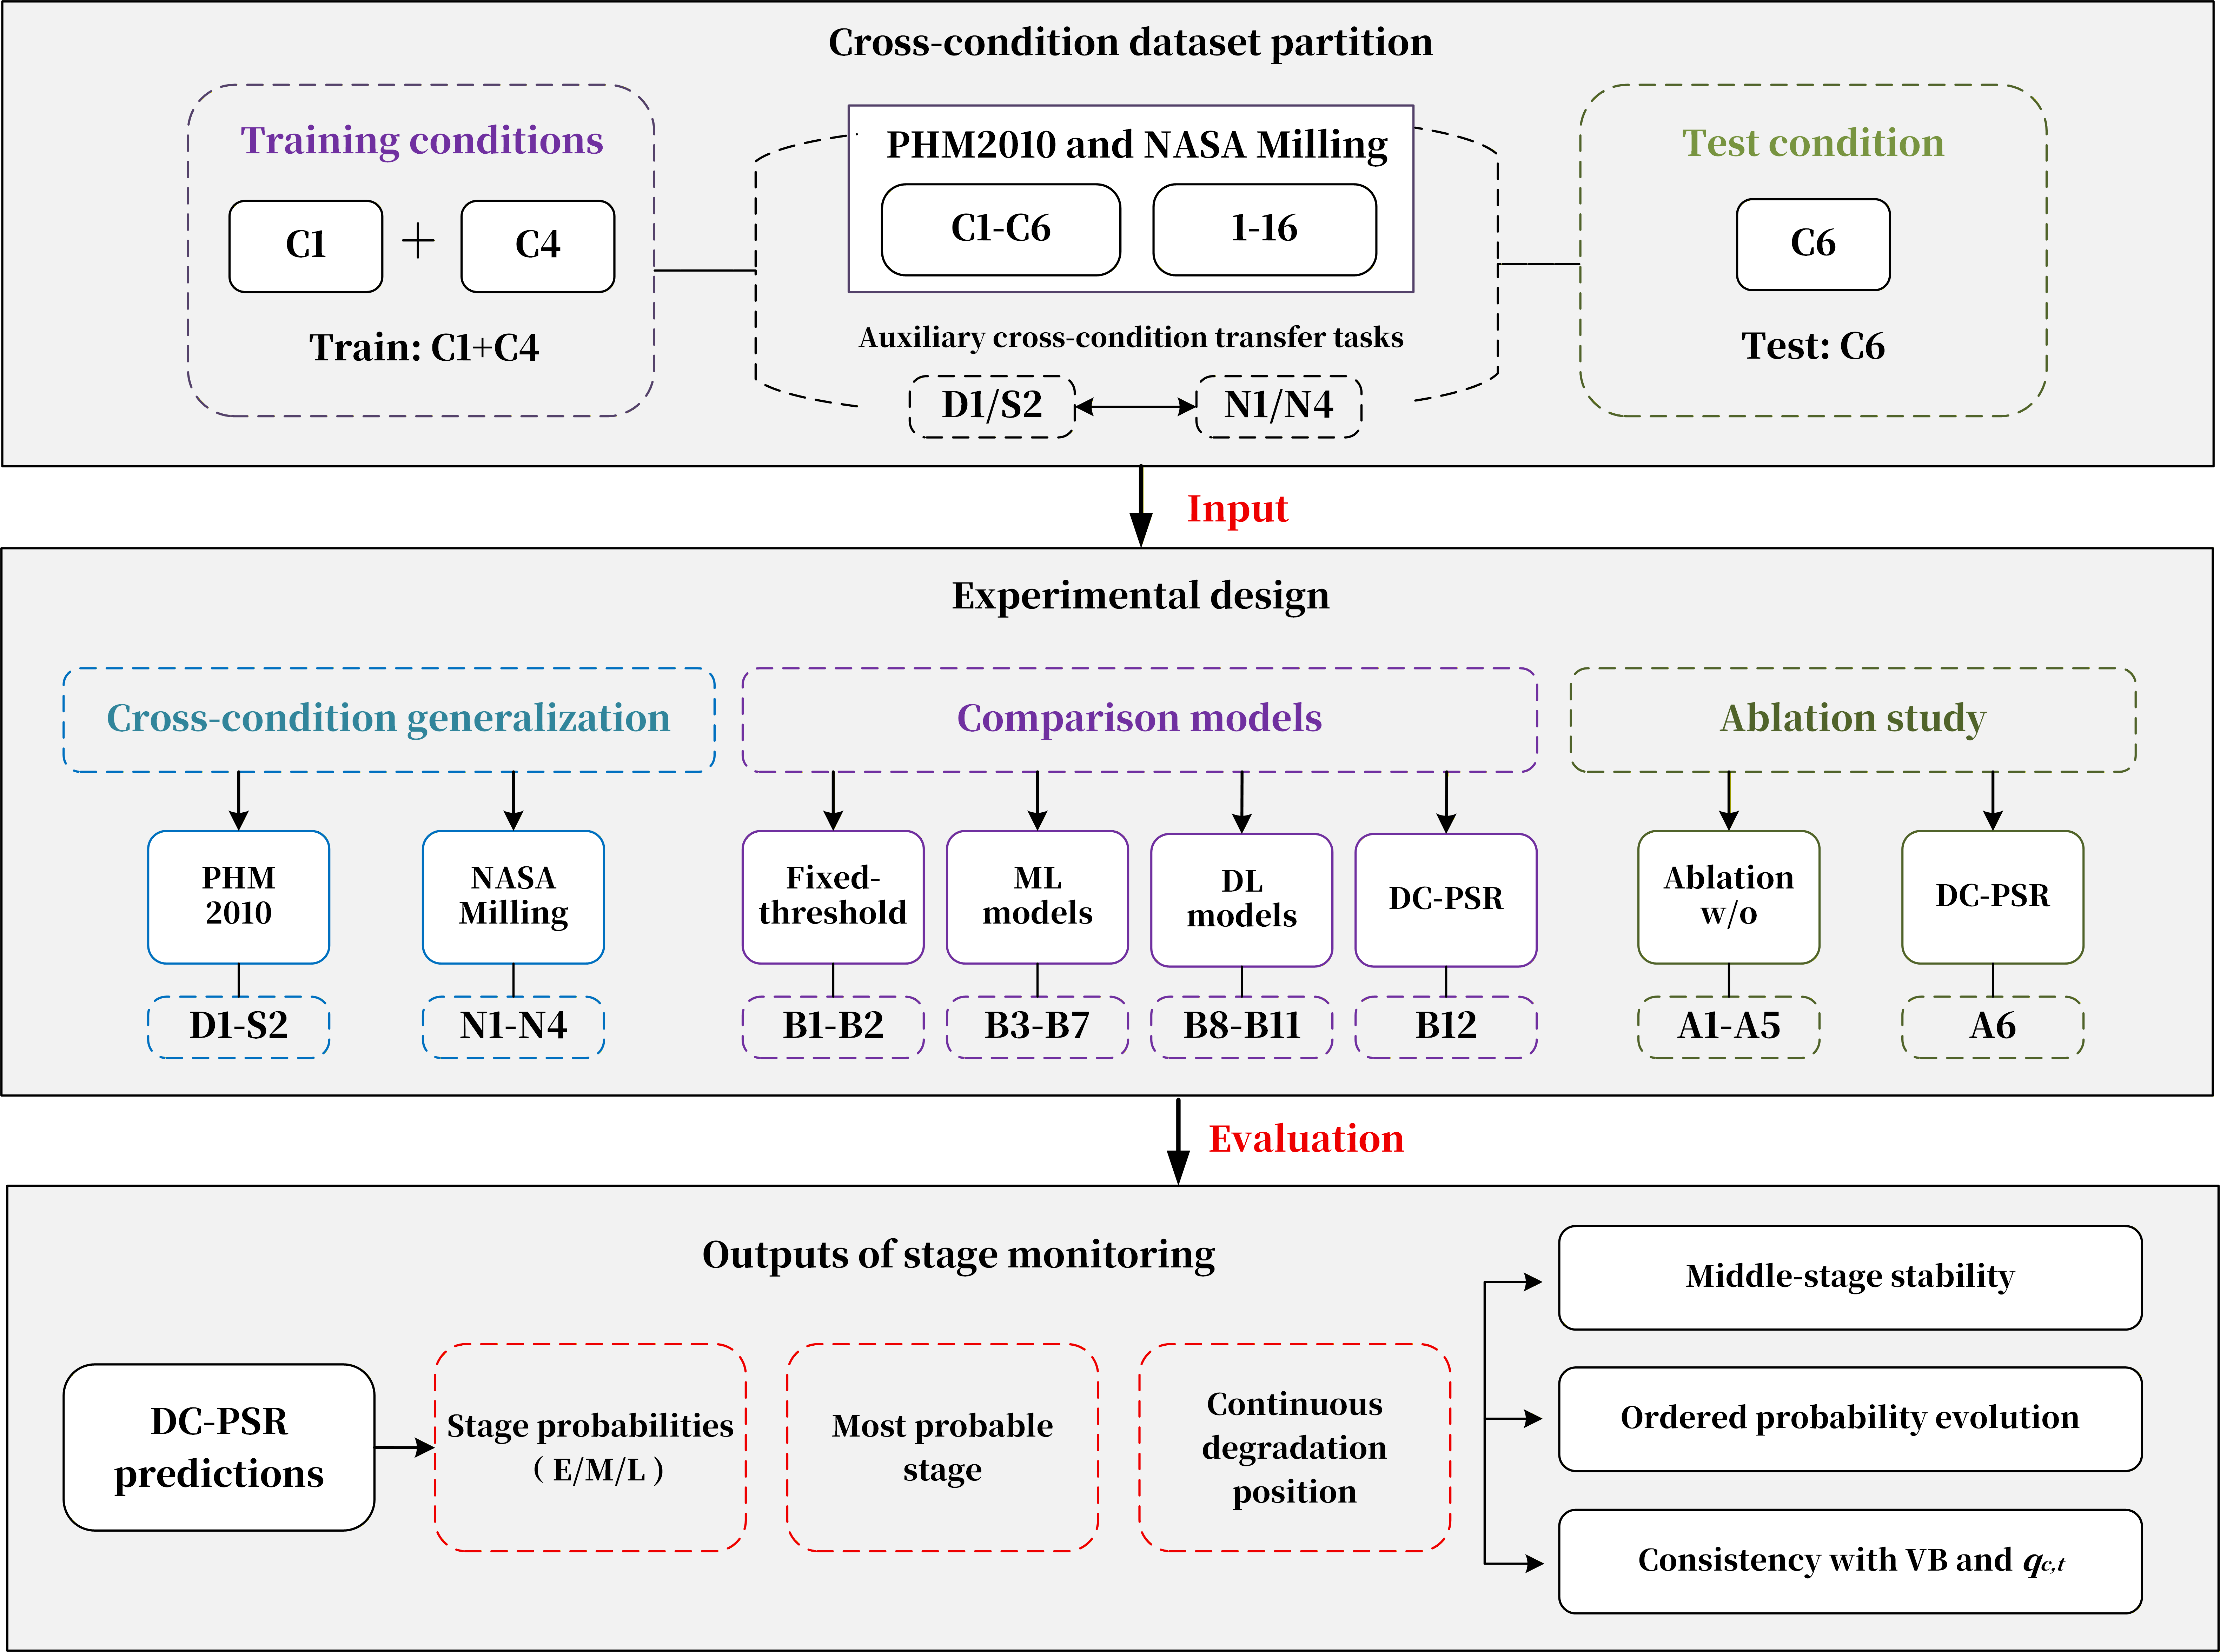
\includegraphics[width=0.85\textwidth,keepaspectratio]{figures/fig7.png}
    \caption{Experimental workflow.}
    \label{fig:7}
  \end{figure}
\FloatBarrier
\section{Experimental Analysis}
\label{sec:results}
  \subsection{Main Comparison Results}
\label{sec:main_results}
  This section compares B1--B12 on the D1 task. The results are reported in \tabref{tab:8}. Beyond classification accuracy, the analysis focuses on middle-stage error direction and stage-probability consistency.

  \begin{table*}[!htbp]
    \centering
    \scriptsize
  \caption{Main comparison results.}
    \label{tab:8}
    \begin{adjustbox}{max width=\textwidth}
      \begin{tabular}{lllllllllllll}
        \toprule
        \textbf{ID} & \textbf{Acc} & \textbf{Macro-F1} & \textbf{E-F1} & \textbf{M-F1} & \textbf{L-F1} & \textbf{M-Pre} & \textbf{M-Rec} & \textbf{$M\rightarrow E$} & \textbf{$M\rightarrow L$} & \textbf{Rev} & \textbf{Jump} & \textbf{Smooth} \\
        \midrule
        B1 & 0.6447 & 0.6145 & 0.4587 & 0.5970 & 0.7879 & 0.5755 & 0.6202 & \textbf{0.0000} & 0.3798 & 0 & 0 &0.0132 \\
        B2 & 0.5757 & 0.4871 & 0.7304 & 0.0000 & 0.7309 & 0.0000 & 0.0000 & 0.4806 & 0.5194 & 5 & 11 & 0.0726 \\
        B3 & 0.9474 & 0.9490 & 0.9231 & 0.9350 & 0.9889 & 0.9829 & 0.8915 & 0.1085 & 0.0000 & 5 & 0 & 0.1096 \\
        B4 & 0.8651 & 0.8695 & 0.8737 & 0.8379 & 0.8970 & 0.8548 & 0.8217 & 0.1783 & 0.0000 & 9 & 0 & 0.1578 \\
        B5 & 0.9770 & 0.9773 & 0.9651 & 0.9723 & 0.9945 & 0.9919 & 0.9535 & 0.0388 & 0.0078 & 5 & 0 & 0.1105 \\
        B6 & 0.8783 & 0.8765 & 0.8054 & 0.8702 & 0.9540 & 0.7949 & 0.9612 & 0.0388 & 0.0000 & 9 & 0 & 0.1390 \\
        B7 & 0.8618 & 0.8651 & 0.8889 & 0.8174 & 0.8889 & 0.9307 & 0.7287 & 0.1628 & 0.1085 & 16 & 0 & 0.1554 \\
        B8 & 0.9539 & 0.9550 & 0.9385 & 0.9426 & 0.9838 & 1.0000 & 0.8915 & 0.0853 & 0.0233 & 10 & 0 & 0.1245 \\
        B9 & 0.9539 & 0.9560 & 0.9825 & 0.9426 & 0.9430 & 1.0000 & 0.8915 & 0.0233 & 0.0853 & 1 & 0 & 0.0398 \\
        B10 & 0.8684 & 0.8746 & 0.8317 & 0.8261 & 0.9659 & 0.9406 & 0.7364 & 0.2636 & 0.0000 & 0 & 0 & 0.0219 \\
        B11 & \textbf{0.9901} & \textbf{0.9902} & 0.9825 & \textbf{0.9882} & \textbf{1.0000} & \textbf{1.0000} & 0.9767 & 0.0233 & 0.0000 & 0 & 0 & 0.0236 \\
        B12 & 0.9868 & 0.9871 & \textbf{0.9825} & 0.9844 & 0.9945 & 0.9921 & \textbf{0.9767} & 0.0233 & \textbf{0.0000} & \textbf{0} & \textbf{0} &  \textbf{0.0188} \\
        \bottomrule
      \end{tabular}
    \end{adjustbox}
  \end{table*}
  As shown in \tabref{tab:8}, rule-based methods perform poorly in cross-condition stage monitoring, indicating that fixed thresholds or simple relative rules are insufficient for stable stage-state representation. Conventional machine-learning and deep temporal models improve classification performance, but still suffer from inadequate middle-stage coverage or fluctuating probabilistic outputs. Some methods achieve high overall accuracy but exhibit large Smooth values, suggesting unstable stage-probability sequences that are unsuitable for continuous state modeling.
  
  Compared with B10 and other single-task temporal models, B11 substantially improves stage discrimination, showing that fine-grained classification and degradation-position estimation enhance the shared degradation representation. B12 achieves slightly lower hard-classification scores than B11, but maintains a high overall level while reducing $M\rightarrow L$ to zero and further decreasing Smooth. This indicates that DC-PSR does not simply maximize hard classification accuracy; instead, it calibrates instantaneous stage outputs into smoother probabilistic states with stronger degradation consistency.

  \figref{fig:8} compares the overall performance of different methods. B12 maintains a strong balance between stage discrimination and probability stability.
  The normalized confusion matrices in \figref{fig:9} support the same conclusion. B12 preserves clear stage boundaries and effectively reduces premature misclassification from the middle stage to the late stage.
  
  \begin{figure}[pos=!htbp]
    \centering
    \includegraphics[width=0.72\textwidth,keepaspectratio]{figures/fig8.png}
    \caption{Overall method comparison.}
    \label{fig:8}
  \end{figure}

  

  \begin{figure}[pos=!htbp]
    \centering
    
\includegraphics[width=0.9\textwidth,keepaspectratio]{figures/fig9.png}
    \caption{Normalized confusion matrices.}
    \label{fig:9}
  \end{figure}
\figref{fig:10} further evaluates middle-stage recognition, misclassification direction, and stage consistency. B12 suppresses premature middle-to-late transitions while keeping Rev and Jump at zero and achieving a low Smooth value. This confirms that ordered probabilistic inference can reduce non-physical transitions and improve temporal consistency of stage probabilities.

  \begin{figure}[pos=!htbp]
    \centering
    \includegraphics[width=0.9\textwidth,keepaspectratio]{figures/fig10.png}
    \caption{Middle-stage and consistency metrics.}
    \label{fig:10}
  \end{figure}
Overall, DC-PSR is advantageous not because it maximizes a single classification metric, but because it jointly improves stage discrimination, middle-stage coverage, and ordered probability evolution.

  \subsection{Cross-Condition Generalization Results}
\label{sec:cross_condition}
  To evaluate the generalization ability of DC-PSR under different transfer difficulties, dual-source and single-source cross-condition tasks are first constructed on PHM2010. B9--B12 are compared, and the results are shown in \tabref{tab:9}.

  \begin{table*}[!htbp]
    \centering
    \scriptsize
  \caption{PHM2010 cross-condition results.}
    \label{tab:9}
    \begin{adjustbox}{max width=\textwidth}
      \begin{tabular}{llllllllll}
        \toprule
        \textbf{Task} & \textbf{Method} & \textbf{Acc} & \textbf{Macro-F1} & \textbf{M-F1} & \textbf{M-Rec} & \textbf{$M\rightarrow E$} & \textbf{$M\rightarrow L$} & \textbf{Rev} & \textbf{Smooth} \\
        \midrule
        D1 & B9 & 0.8026 & 0.8013 & 0.6970 & 0.5349 & 0.2713 & 0.1938 & 1 & 0.0300 \\
        & B10 & 0.7928 & 0.7904 & 0.6769 & 0.5116 & 0.2713 & 0.2171 & 1 & 0.0391 \\
        & B11 & \textbf{0.9868} & \textbf{0.9871} & \textbf{0.9844} & 0.9767 & 0.0233 & 0.0000 & 0 & 0.0247 \\
        & B12 & 0.9836 & 0.9840 & 0.9805 & \textbf{0.9767} & \textbf{0.0233} & \textbf{0.0000} & \textbf{0} & \textbf{0.0192} \\
        D2 & B9 & 0.8816 &0.8840 & 0.8407 & 0.8559 & 0.0000 & 0.1441 & 0 & 0.0152 \\
        & B10 & \textbf{0.8816} & \textbf{0.8840} & \textbf{0.8407} & \textbf{0.8559} & 0.0000 & \textbf{0.1441} & 0 & 0.0186 \\
        & B11 & 0.8553 & 0.8575 & 0.7963 & 0.7748 & 0.0000 & 0.2252 & 0 & \textbf{0.0136} \\
        & B12 & 0.8651 & 0.8674 & 0.8128 & 0.8018 & \textbf{0.0000} & 0.1982 & \textbf{0} & 0.0145 \\
        S1 & B9 & 0.8849 & 0.8869 & 0.8416 & 0.8378 & 0.0090 & 0.1532 & 1 & 0.0232 \\
        & B10 & 0.9145 & 0.9177 & 0.8898 & 0.9459 & 0.0180 & 0.0360 & 1 & 0.0208 \\
        & B11 & 0.9145 & 0.9172 & 0.8898 & 0.9459 & 0.0000 & 0.0541 & 0 & 0.0144 \\
        & B12 & \textbf{0.9243} & \textbf{0.9271} & \textbf{0.9030} & \textbf{0.9640} & \textbf{0.0000} & \textbf{0.0360} & \textbf{0} & \textbf{0.0134} \\
        S2 & B9 & 0.7961 & 0.8017 & 0.6837 & 0.6036 & 0.3333 & 0.0631 & 2 & 0.0412 \\
        & B10 & 0.8816 & 0.8846 & 0.8571 & 0.9730 & 0.0000 & 0.0270 & 0 & 0.0185 \\
        & B11 & \textbf{0.9375} & \textbf{0.9406} & \textbf{0.9212} & 0.9876 & 0.0000 & 0.0000 & 0 & 0.0196 \\
        & B12 & 0.9309 & 0.9341 & 0.9136 & \textbf{1.0000} & \textbf{0.0000} & \textbf{0.0000} & \textbf{0} & \textbf{0.0144} \\
        \bottomrule
      \end{tabular}
    \end{adjustbox}
  \end{table*}
  \tabref{tab:9} shows that B9 and B10 exhibit noticeable fluctuations across transfer tasks, especially in D1 and S2, where middle-stage recall is insufficient. This suggests that single temporal networks can capture certain degradation patterns, but their stage semantics remain unstable when source and target conditions differ substantially. In contrast, B11 and B12 achieve stronger overall performance, indicating that fine-grained state classification and continuous degradation-position estimation improve cross-condition stage representation.

  A further comparison between B11 and B12 shows that their classification metrics are close in most tasks, whereas B12 usually achieves lower Smooth and fewer reverse transitions. This demonstrates that the advantage of DC-PSR is not limited to improving pointwise classification accuracy. More importantly, it calibrates instantaneous stage outputs into smoother probabilistic states that better follow the degradation order.

  \tabref{tab:10} reports the mean and standard deviation over the four PHM2010 cross-condition tasks. B12 achieves the best average results across all listed metrics, indicating both strong mean generalization performance and reduced variability in stage-probability evolution.

  \begin{table}[!htbp]
    \centering
    \scriptsize
  \caption{Average cross-condition performance.}
    \label{tab:10}
    \begin{adjustbox}{max width=\textwidth}
      \begin{tabular}{llllll}
        \toprule
        \textbf{Method} & \textbf{Acc} & \textbf{Macro-F1} & \textbf{M-F1} & \textbf{M-Rec} & \textbf{Smooth} \\
        \midrule
        B9 & 0.8413 $\pm$ 0.0485 & 0.8435 $\pm$ 0.0485 & 0.7658 $\pm$ 0.0817 & 0.7080 $\pm$ 0.1629 & 0.0272 $\pm$ 0.0113 \\
        B10 & 0.8676 $\pm$ 0.0522 & 0.8692 $\pm$ 0.0548 & 0.8161 $\pm$ 0.0947 & 0.8216 $\pm$ 0.2126 & 0.0243 $\pm$ 0.0100 \\
        B11 & 0.9235 $\pm$ 0.0546 & 0.9256 $\pm$ 0.0539 & 0.8980 $\pm$ 0.0792 & 0.9244 $\pm$ 0.1022 & 0.0181 $\pm$ 0.0052 \\
        B12 & \textbf{0.9260 $\pm$ 0.0485} & \textbf{0.9281 $\pm$ 0.0478} & \textbf{0.9025 $\pm$ 0.0714} & \textbf{0.9356 $\pm$ 0.0905} & \textbf{0.0156 $\pm$ 0.0025} \\
        \bottomrule
      \end{tabular}
    \end{adjustbox}
  \end{table}
  \figsref{fig:11}{fig:13} further support these findings from different perspectives.

  \begin{figure}[pos=!htbp]
    \centering
    \includegraphics[width=0.9\textwidth,keepaspectratio]{figures/fig11.png}
    \caption{DC-PSR confusion matrices across conditions.}
    \label{fig:11}
  \end{figure}
\figref{fig:11} shows that DC-PSR maintains clear stage boundaries under typical cross-condition settings. \figref{fig:12} presents the evolution of stage probabilities along the tool life cycle, indicating that the output probabilities carry explicit life-cycle semantics. \figref{fig:13} further shows that DC-PSR improves mean performance while reducing cross-task variability.

  \begin{figure}[pos=!htbp]
    \centering
    \includegraphics[width=0.9\textwidth,keepaspectratio]{figures/fig12.png}
    \caption{Stage partitioning and probability evolution.}
    \label{fig:12}
  \end{figure}

  \begin{figure}[pos=!htbp]
    \centering
    \includegraphics[width=0.9\textwidth,keepaspectratio]{figures/fig13.png}
    \caption{Mean and variability of cross-condition performance.}
    \label{fig:13}
  \end{figure}
To further examine the applicability of DC-PSR under external small-sample, multi-case conditions, candidate cross-case tasks are constructed on NASA Milling. The results are shown in \tabref{tab:11}.

  \begin{table*}[!htbp]
    \centering
    \scriptsize
  \caption{NASA external cross-case results.}
    \label{tab:11}
    \begin{adjustbox}{max width=\textwidth}
      \begin{tabular}{llllllllll}
        \toprule
        \textbf{Task} & \textbf{Method} & \textbf{Acc} & \textbf{Macro-F1} & \textbf{M-F1} & \textbf{M-Rec} & \textbf{$M\rightarrow E$} & \textbf{$M\rightarrow L$} & \textbf{Rev} & \textbf{Smooth} \\
        \midrule
        N1 & B9 & 0.5385 & 0.5713 & 0.4545 & 0.3571 & 0.0714 & 0.5714 & 1 & 0.1462 \\
        & B10 & 0.5000 & 0.4179 & 0.6047 & 0.6842 & 0.1053 & 0.2632 & 1 & 0.1834 \\
        & B11 & 0.7059 & \textbf{0.7019} & 0.7300 & 0.7895 & 0.1053 & 0.1053 & 2 & 0.3315 \\
        & B12 & \textbf{0.7059} & 0.6873 & \textbf{0.7619} & \textbf{0.8421} & \textbf{0.0526} & \textbf{0.0526} & \textbf{0} & \textbf{0.0563} \\
        N2 & B9 & 0.4074 & 0.3638 & 0.2222 & 0.5000 & 0.5000 & 0.0000 & 1 & 0.0737 \\
        & B10 & 0.5161 & 0.3761 & 0.0000 & 0.0000 & 0.5000 & 0.5000 & 1 & 0.1451 \\
        & B11 & 0.7037 & 0.6455 & 0.5000 & 0.5000 & 0.5000 & 0.0000 & 1 & 0.1781 \\
        & B12 & \textbf{0.7163} & \textbf{0.6895} & \textbf{0.6270} & \textbf{0.6305} & \textbf{0.5000} & \textbf{0.0000} & \textbf{0} & \textbf{0.0562} \\
        N3 & B9 & 0.4848 & 0.4675 & 0.4286 & 0.3750 & 0.1250 & 0.5000 & 2 & 0.0797 \\
        & B10 & 0.4242 & 0.4334 & 0.5714 & 0.7500 & 0.1250 & 0.2222 & 4 & 0.1302 \\
        & B11 & 0.6676 & 0.6952 & 0.5167 & 0.6556 & 0.1111 & 0.3333 & 1 & 0.1561 \\
        & B12 & \textbf{0.7946} & \textbf{0.7720} & \textbf{0.7800} & \textbf{0.7667} & \textbf{0.1002} & \textbf{0.1250} & \textbf{0} & \textbf{0.0116} \\
        N4 & B9 & 0.4706 & 0.4180 & 0.1429 & 0.0769 & 0.8462 & 0.0769 & 1 & 0.2211 \\
        & B10 & 0.4706 & 0.4651 & 0.3810 & 0.3077 & 0.6923 & 0.0000 & 0 & 0.0670 \\
        & B11 & 0.6667 & 0.5810 & 0.6897 & 0.8151 & 0.1297 & 0.0000 & 1 & 0.0805 \\
        & B12 & \textbf{0.6867} & \textbf{0.6956} & \textbf{0.7667} & \textbf{0.9091} & \textbf{0.0909} & \textbf{0.0000} & \textbf{0} & \textbf{0.0582} \\
        \bottomrule
      \end{tabular}
    \end{adjustbox}
  \end{table*}
  As shown in \tabref{tab:11}, DC-PSR remains applicable under external cross-case settings. Compared with B9--B11, B12 generally improves middle-stage recognition and substantially reduces Rev and Smooth, indicating that degradation-consistent constraints can suppress stage jumps and improve probability continuity under small-sample, multi-case conditions. However, NASA Milling contains limited samples per case, and its cases differ in material, cutting parameters, and stage distributions. Therefore, these results are better interpreted as external complementary validation rather than a replacement for the PHM2010 main benchmark.

  \figref{fig:14} summarizes the comprehensive performance of different methods. The results show that DC-PSR still improves middle-stage recognition and probability smoothness on more difficult external data, although its stability is affected by the limited data scale and case heterogeneity.

  \begin{figure}[pos=!htbp]
    \centering
    \includegraphics[width=0.9\textwidth,keepaspectratio]{figures/fig14.png}
    \caption{Radar comparison across transfer tasks.}
    \label{fig:14}
  \end{figure}
Overall, DC-PSR provides a more stable probabilistic stage representation across different transfer difficulties. Its advantage lies not only in classification improvement, but also in the joint enhancement of middle-stage coverage, stage-jump suppression, and probability-evolution continuity.

  \subsection{Ablation Results}
\label{sec:ablation}
  To analyze the contribution of each module, ablation experiments are conducted by focusing on the effects of fine-grained state assistance, degradation-position prior, and ordered probabilistic inference on stage discrimination and probability-evolution stability. The results are shown in \tabref{tab:12}.

  \begin{table*}[!htbp]
    \centering
    \scriptsize
  \caption{Ablation results.}
    \label{tab:12}
    \begin{adjustbox}{max width=\textwidth}
      \begin{tabular}{lllllllll}
        \toprule
        \textbf{ID} & \textbf{Acc} & \textbf{Macro-F1} & \textbf{E-F1} & \textbf{M-F1} & \textbf{L-F1} & \textbf{M-Pre} & \textbf{M-Rec} & \textbf{Smooth} \\
        \midrule
        A1 & 0.9705 & 0.9601 & 0.9625 & 0.9532 & 0.9880 & 0.9852 & 0.9561 & 0.0236 \\
        A2 & 0.9803 & 0.9732 & 0.9678 & 0.9772 & 0.9778 & 0.9834 & 0.9663 & 0.0199 \\
        A3 & 0.9816 & 0.9772 & 0.9725 & 0.9782 & 0.9876 & 0.9889 & 0.9678 & 0.0209 \\
        A4 & \textbf{0.9901} & \textbf{0.9902} & 0.9825 & \textbf{0.9882} & \textbf{1.0000} & \textbf{1.0000} & 0.9767 & 0.0236 \\
        A5 & 0.9770 & 0.9775 & 0.9711 & 0.9725 & 0.9889 & 0.9841 & 0.9612 & \textbf{0.0146} \\
        A6 & 0.9868 & 0.9871 & \textbf{0.9825} & 0.9844 & 0.9945 & 0.9921 & \textbf{0.9767} & 0.0188 \\
        \bottomrule
      \end{tabular}
    \end{adjustbox}
  \end{table*}
  \tabref{tab:12} shows that A1, which uses only the stage classification head, already provides a strong baseline, but the middle stage still has room for improvement. Adding fine-grained state assistance improves both overall performance and M-F1, confirming that ordered fine-grained states provide useful internal structure for stable wear representation. Incorporating the degradation-position prior further improves A3, indicating that continuous degradation position constrains stage-boundary judgment effectively. A4 achieves the highest classification accuracy, suggesting strong complementarity among multiple degradation-related information sources.

  However, the highest hard-classification accuracy does not necessarily imply the best probabilistic stage representation. Although A4 achieves the strongest classification scores, its Smooth remains relatively high. In contrast, A5 substantially reduces Smooth through ordered filtering, but its Acc and M-F1 decrease compared with A4, indicating that overly strong ordering constraints may delay boundary response.

  \figref{fig:15} compares the classification performance of different ablation methods. A6 achieves a better balance between accuracy and smoothness: it maintains high classification performance while keeping Smooth at a low level. This demonstrates that the final fusion strategy improves probability-evolution consistency without sacrificing stage discrimination.

  \begin{figure}[pos=!htbp]
    \centering
    \includegraphics[width=0.8\textwidth,keepaspectratio]{figures/fig15.png}
    \caption{Ablation classification performance.}
    \label{fig:15}
  \end{figure}
\figref{fig:16} further illustrates the trade-off between accuracy and smoothness. Pursuing instantaneous classification accuracy alone may lead to probability fluctuations, whereas relying excessively on ordered filtering may cause boundary lag. Therefore, the performance gain of DC-PSR comes from the coordinated effect of fine-grained states, degradation-position priors, and ordered probabilistic inference: the first two enhance stage discrimination and internal structure modeling, while the last constrains stage probabilities to evolve stably along the tool life cycle.

  \begin{figure}[pos=!htbp]
    \centering
    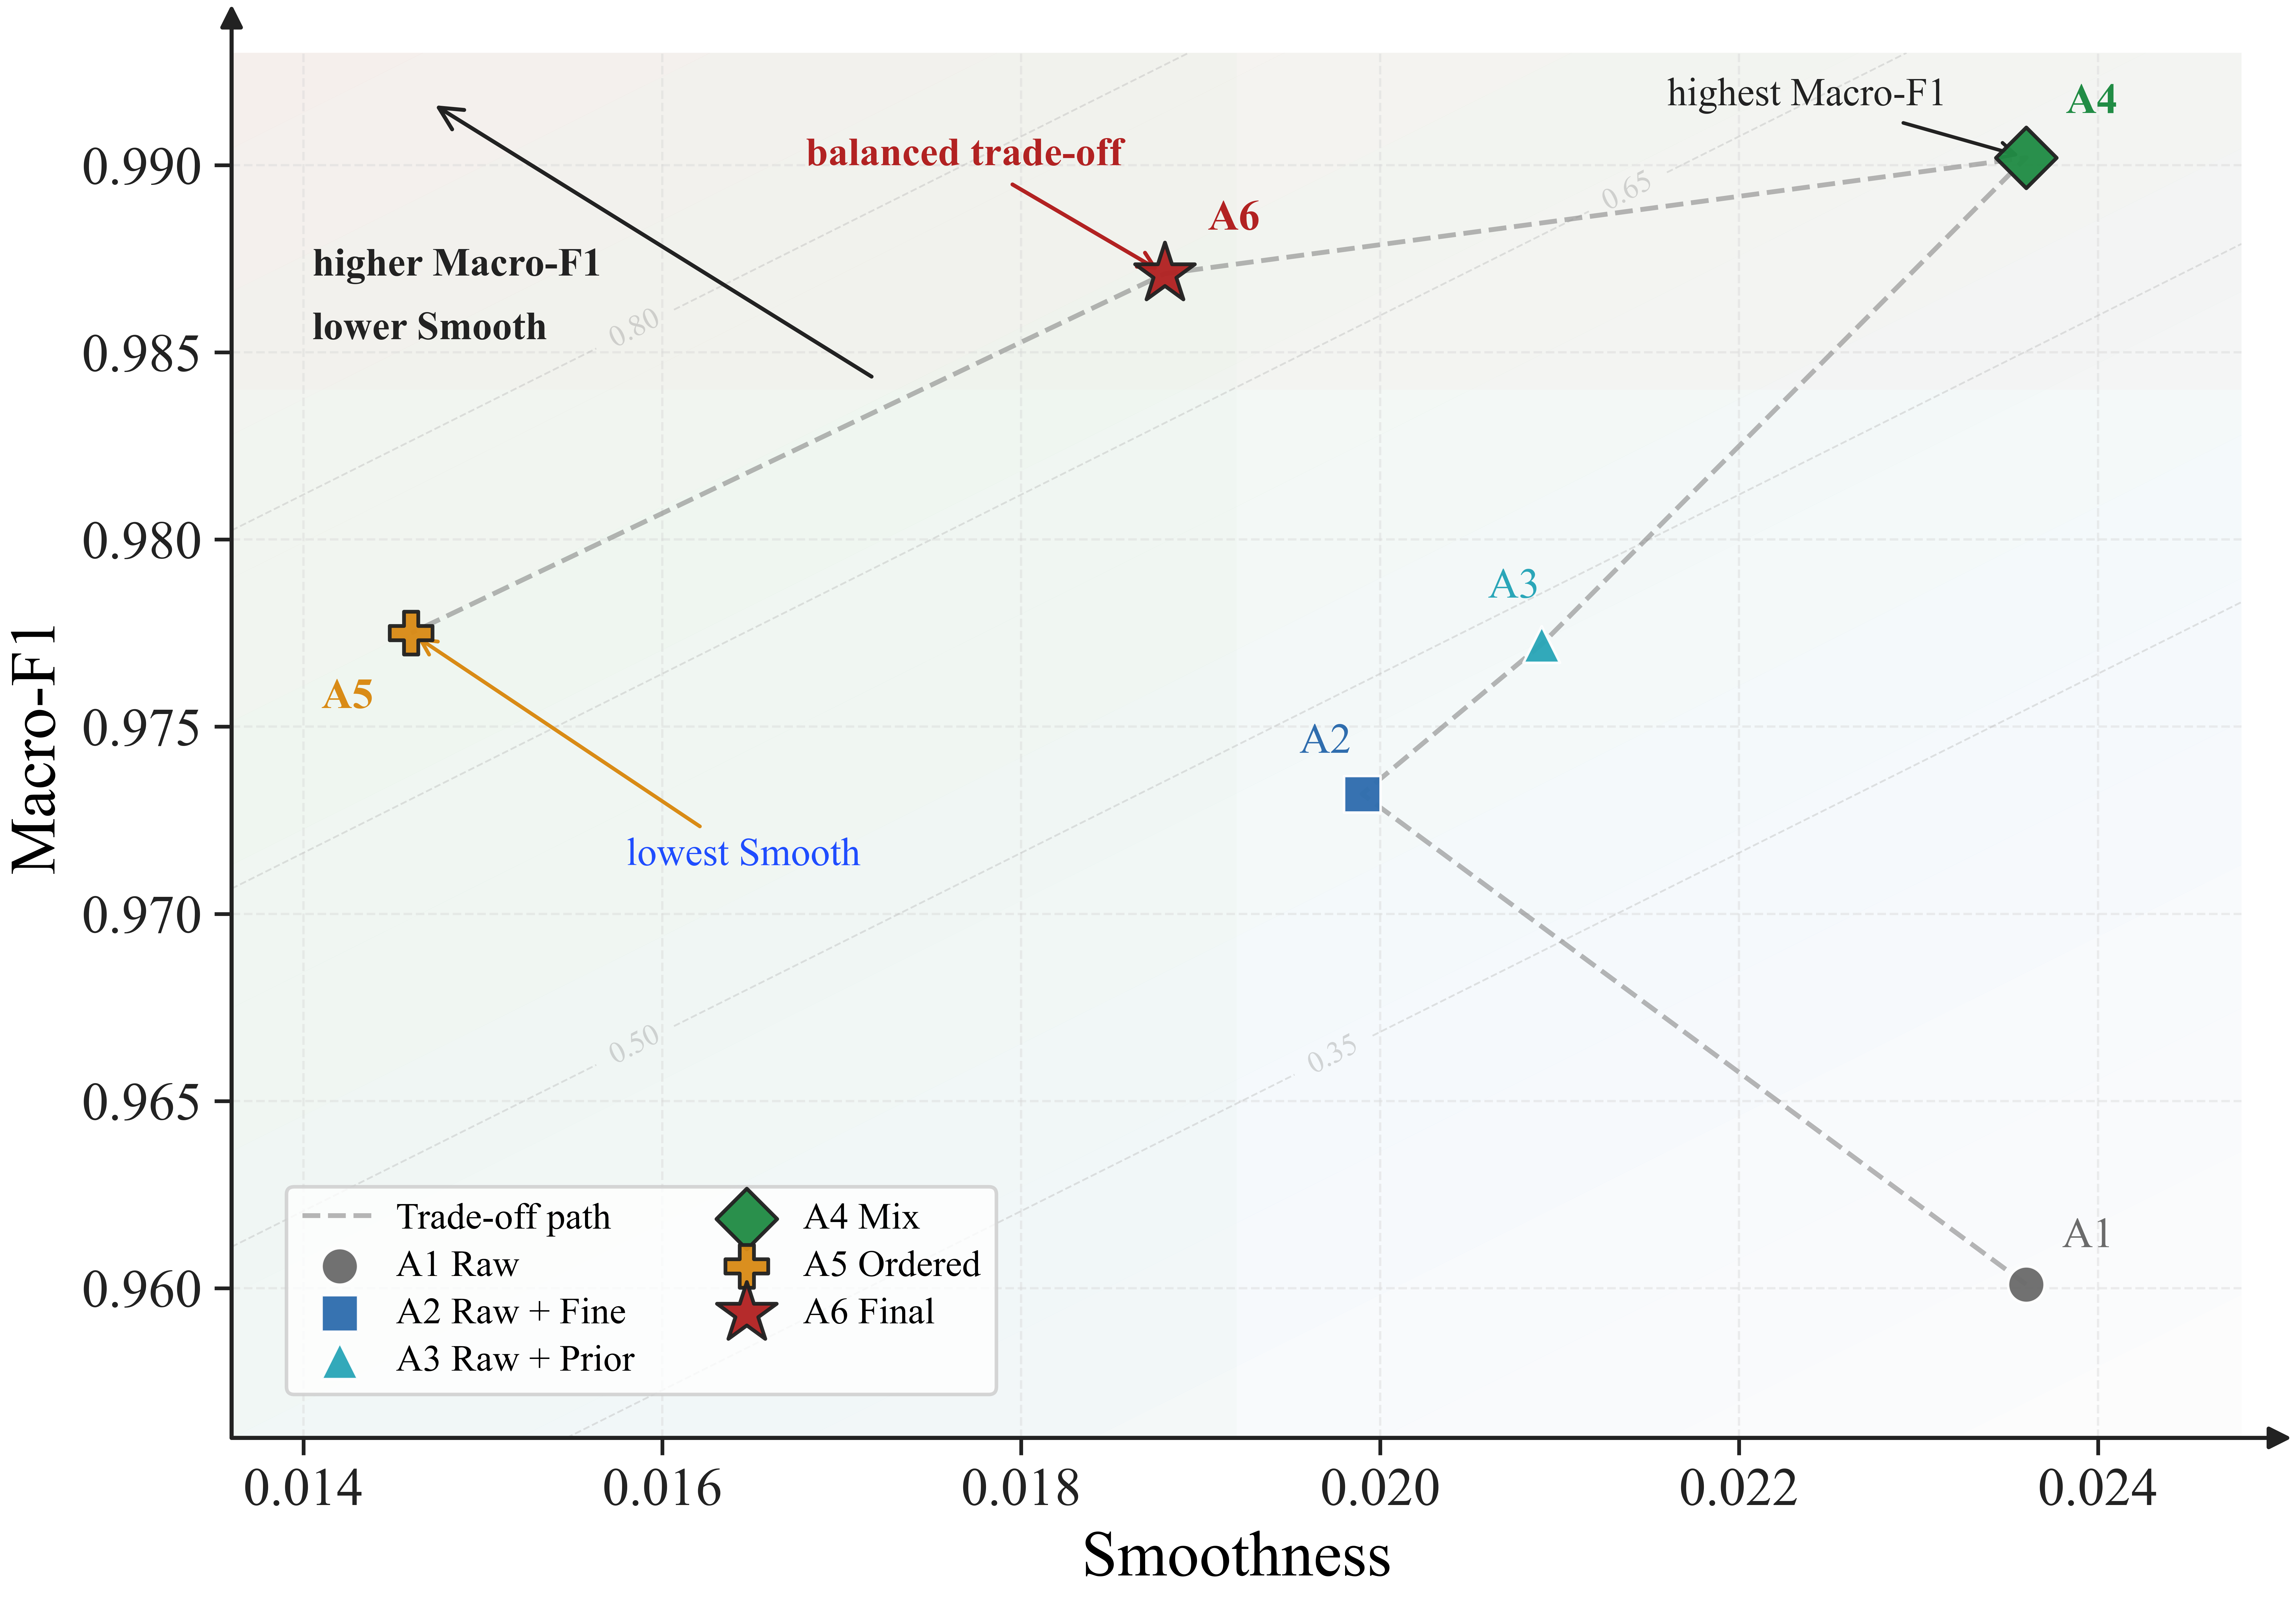
\includegraphics[width=0.6\textwidth,keepaspectratio]{figures/fig16.png}
    \caption{Accuracy--smoothness trade-off.}
    \label{fig:16}
  \end{figure}
\subsection{Wear-Estimation Consistency Analysis}
\label{sec:wear_consistency}
  To examine whether the proposed method carries actual wear semantics, the consistency between the estimated degradation position $\hat{q}_{c,t}$ and the true relative degradation position $q_{c,t}$ is analyzed. The degradation positions and wear levels under different predicted stages are also summarized in \tabsref{tab:13}{tab:14}.

  \begin{table}[!htbp]
    \centering
    \scriptsize
  \caption{Degradation-position estimation results.}
    \label{tab:13}
    \begin{adjustbox}{max width=\textwidth}
      \begin{tabular}{lllllll}
        \toprule
        \textbf{Dataset} & \textbf{$q$-MAE} & \textbf{$q$-RMSE} & \textbf{$q$-$R^2$} & \textbf{Spearman} & \textbf{Pearson} & \textbf{$q$-Smooth} \\
        \midrule
        PHM2010 & 0.1252 & 0.1590 & 0.8672 & 0.9635 & 0.9388 & 0.0082 \\
        NASA Milling & 0.1784 & 0.2087 & 0.7087 & 0.8136 & 0.7959 & 0.0616 \\
        \bottomrule
      \end{tabular}
    \end{adjustbox}
  \end{table}
  \tabref{tab:13} shows that $\hat{q}_{c,t}$ is highly consistent with $q_{c,t}$. The low $q$-Smooth values further indicate that the estimated degradation position evolves smoothly, providing a stable degradation scale for probabilistic stage inference.

  \tabref{tab:14} shows a monotonic increase in $\hat{q}_{c,t}$, $q_{c,t}$, and VB from early to middle and late. This confirms that the stage output of DC-PSR is not an isolated classification result, but a degradation-semantic representation aligned with actual wear levels and continuous degradation positions.

  \begin{table}[!htbp]
    \centering
    \scriptsize
  \caption{Wear semantics of predicted stages.}
    \label{tab:14}
    \begin{adjustbox}{max width=\textwidth}
      \begin{tabular}{llll}
        \toprule
        \textbf{Predicted stage} & \textbf{Mean $q_{c,t}$} & \textbf{Mean $\hat{q}_{c,t}$} & \textbf{Mean $VB$} \\
        \midrule
        early & 0.2110 & 0.2248 & 100.55 \\
        middle & 0.3629 & 0.3444 & 126.29 \\
        late & 0.8289 & 0.8451 & 205.46 \\
        \bottomrule
      \end{tabular}
    \end{adjustbox}
  \end{table}
  To further evaluate representation capability, two-dimensional PCA visualization is performed on the raw online relative features and the shared hidden representation $\mathbf{h}_{c,t}$, as shown in \figref{fig:17}. In the raw feature space, samples from different stages overlap and are scattered along the degradation position $q$. In contrast, the shared hidden representation forms clearer stage separation and a more continuous degradation trajectory, indicating that the model jointly encodes stage-discrimination information, continuous degradation position, and boundary uncertainty.

  \begin{figure}[pos=!htbp]
    \centering
    \includegraphics[width=0.9\textwidth,keepaspectratio]{figures/fig17.png}
    \caption{Low-dimensional feature representations.}
    \label{fig:17}
  \end{figure}
\figref{fig:18} further presents the joint evolution of stage probabilities and $\hat{q}_{c,t}$ along the tool life cycle. Overall, DC-PSR produces stage probabilities that are not only accurate and temporally smooth, but also consistent with continuous degradation position and actual wear level. Therefore, the proposed method forms a degradation state representation supported by explicit wear semantics.

  \begin{figure}[pos=!htbp]
    \centering
    \includegraphics[width=0.9\textwidth,keepaspectratio]{figures/fig18.png}
    \caption{Joint evolution of stage probability and degradation position.}
    \label{fig:18}
  \end{figure}
\FloatBarrier
\section{Discussion}
\label{sec:discussion}
  The primary challenge in cross-condition stage representation is stage semantic drift. Under different cutting conditions, wear magnitude, growth rate, and failure boundary may vary substantially. If stages are directly defined by absolute thresholds, the model tends to learn condition-specific wear intervals rather than relative degradation states within the tool life cycle. More importantly, stage semantic drift can also weaken the reliability of continuous degradation representation: when the same wear level corresponds to different signal scales across conditions, the model may exhibit different bias patterns at different stages. DC-PSR addresses this issue by constructing stage semantics from condition-relative degradation positions and local degradation rates. In this way, absolute wear levels are transformed into relative degradation processes, providing a more consistent semantic basis for cross-condition stage representation.

  The middle stage is the most easily simplified and misclassified part of wear stage monitoring. The stable wear period usually contains a continuous transition from early stable wear to later accelerated degradation. By introducing ordered fine-grained degradation states, DC-PSR provides internal hierarchical support for the middle stage, enabling the model to learn not only stage boundaries but also progressive variations within stable wear. The ablation results show that fine-grained state assistance significantly improves middle-stage recognition, confirming that the middle stage should be modeled as a structured degradation process rather than a simple intermediate label.

  The goal of probabilistic stage representation is to generate a state distribution that can be continuously updated along the degradation process. Multi-task TCN-GRU is closer to an instantaneous discrimination optimum, whereas DC-PSR is closer to a degradation-state representation optimum. The former improves current-stage recognition through auxiliary tasks, while the latter further uses degradation-position priors, dual-side inhibition, and causal ordered filtering to calibrate instantaneous probabilities into smoothly evolving stage states. The results show that DC-PSR maintains strong discrimination performance while reducing Smooth and suppressing unreasonable misclassifications. Its advantage therefore lies in balancing stage accuracy, temporal stability, and degradation-evolution consistency.

  The wear-estimation consistency analysis further indicates that the stage probabilities generated by DC-PSR are not isolated classification confidences, but state representations with continuous wear semantics. Across different predicted stages, the probabilistic states produced by DC-PSR remain consistent with actual wear levels and degradation directions. The low-dimensional representation visualization also shows that, compared with raw online relative features, the shared hidden representation $\mathbf{h}_{c,t}$ forms clearer stage separation and a more continuous degradation trajectory along the life cycle. These results suggest that DC-PSR has the potential to support stage-aware RUL prediction and predictive maintenance decision-making.

  Nevertheless, DC-PSR still assumes that tool wear follows a relatively clear progressive degradation trend. In cases of sudden chipping, strongly interrupted cutting, or abrupt changes in wear mechanisms, an overly strong ordered-stage prior may delay the response to rapid state changes. In addition, the experiments are mainly conducted on PHM2010 and NASA Milling. Future work should validate the robustness of DC-PSR on broader tool types, workpiece materials, and industrial field data, and further explore stage-probability-driven RUL distribution prediction models.

  \section{Conclusions}
\label{sec:conclusions}
  This paper proposed DC-PSR for cross-condition tool wear monitoring, aiming to address stage semantic drift, middle-stage compression, stage-related bias, and unstable probabilistic outputs. The method constructs relative stage semantics, introduces ordered fine-grained degradation states, and integrates degradation-position priors with causal ordered filtering. In this way, conventional hard stage classification is reformulated as degradation-consistent probabilistic state representation along the tool life cycle.

  Experiments on PHM2010 show that DC-PSR achieves strong cross-condition stage discrimination while improving middle-stage coverage, suppressing non-physical transitions, and smoothing stage probabilities. External validation on NASA Milling further indicates that DC-PSR remains effective under small-sample, multi-case conditions, although its stability is affected by data scale and case heterogeneity. Ablation results verify that fine-grained state assistance, degradation-position priors, and ordered inference contribute complementary benefits in terms of internal stage structure, position consistency, and temporal order. Wear-estimation consistency analysis further shows that the stage probabilities produced by DC-PSR are not merely classification confidences, but degradation-state representations aligned with continuous degradation position, actual wear level, and stage-related representation reliability.

  Overall, DC-PSR advances cross-condition tool wear st age modeling from discrete category recognition to degradation-consistent probabilistic representation, providing a continuously updateable state basis for stage-aware decision-making. Future work will validate the method on broader tool types, workpiece materials, and industrial field data, and explore learnable stage-transition mechanisms and stage-probability-driven RUL prediction.
  
\section*{CRediT authorship contribution statement}
\textbf{Ting Wang}: Conceptualization, Methodology, Software, Validation, Formal analysis, Investigation, Writing -- original draft, Visualization. 
\textbf{Jiali Cheng}: Methodology, Validation, Writing -- review \& editing. 
\textbf{Rongze Li}: Data curation, Software, Validation, Visualization. 
\textbf{Zhenggeng Ye}: Formal analysis, Writing -- review \& editing. 
\textbf{Keqin Wang}: Funding acquisition, Resources, Writing -- review \& editing. 
\textbf{Zhiqiang Cai}: Supervision, Project administration, Resources, Writing -- review \& editing.

\section*{Funding} This work was supported by the Key Project of the Natural Science Foundation of Shaanxi Province (Grant No. 2025JC-QYXQ-043) and the Natural Science Foundation of Shaanxi Province (Grant No. 2025JC-YBMS-807). 

\section*{Data availability}
The PHM2010 dataset is publicly available at \href{https://www.kaggle.com/datasets/rabahba/phm-data-challenge-2010}{https://www.kaggle.com/datasets/rabahba/phm-data-challenge-2010}. The NASA Milling dataset is publicly available from the NASA Prognostics Center of Excellence data repository at \href{https://www.nasa.gov/intelligent-systems-division/discovery-and-systems-health/pcoe/pcoe-data-set-repository/}{https://www.nasa.gov/intelligent-systems-division/discovery-and-systems-health/pcoe/pcoe-data-set-repository/}. The processed data and implementation details are available from the corresponding author upon reasonable request.

  \begin{thebibliography}{99}
    \bibitem[Bernini et~al.(2023)]{ref1} Bernini, L., Albertelli, P., \& Monno, M. (2023). Mill condition monitoring based on instantaneous identification of specific force coefficients under variable cutting conditions. Mechanical Systems and Signal Processing, 185, 109820.
    \bibitem[Bernini et~al.(2024)]{ref2} Bernini, L., Malguzzi, U., Albertelli, P., et al. (2024). Hybrid prognostics to estimate cutting inserts remaining useful life based on direct wear observation. Mechanical Systems and Signal Processing, 210, 111163.
    \bibitem[Cao et~al.(2025)]{ref3} Cao, F., Zhang, X., Zhang, Z., et al. (2025). Research on dynamic graph isomorphism network for tool wear stage monitoring based on multi-source information fusion. Measurement, 119007.
    \bibitem[Cheng et~al.(2026)]{ref4} Cheng, J., Wang, Y., Li, B., et al. (2026). Mutual information-guided causal feature selection method for quality prediction of complex products. Reliability Engineering \& System Safety, 112536.
    \bibitem[Cheng et~al.(2022)]{ref5} Cheng, M., Jiao, L., Yan, P., et al. (2022). Intelligent tool wear monitoring and multi-step prediction based on deep learning model. Journal of Manufacturing Systems, 62, 286--300.
    \bibitem[Dong et~al.(2026)]{ref6} Dong, X., Liu, S., Li, X., et al. (2026). Tool wear trend prediction using acoustic emission signals: A composite multiscale fractional diversity entropy approach. Results in Engineering, 110719.
    \bibitem[Feng et~al.(2026)]{ref7} Feng, C., Ye, H., Li, W., et al. (2026). A hybrid model for tool wear monitoring via physics-based and data-driven utilizing unscented Kalman filter. Advanced Engineering Informatics, 72, 104448.
    \bibitem[Han et~al.(2026)]{ref8} Han, Z., Luo, W., Liang, X., et al. (2026). Online dynamic parameter calibration of a physics-driven hybrid model for tool wear prediction. Journal of Manufacturing Systems, 86, 676--693.
    \bibitem[Heydarlou et~al.(2026)]{ref9} Heydarlou, M. M., Araghizad, A. E., Yamada, Y., et al. (2026). On-machine tool wear monitoring system using strain-gauge signals and edge force coefficients with physics-informed machine learning. CIRP Annals.
    \bibitem[Huang et~al.(2026)]{ref10} Huang, J., Liu, K., Jiang, Y., et al. (2026). Cascaded self-attention hybrid model for synergistic prediction of tool wear and classification of surface roughness in the turning process. Mechanical Systems and Signal Processing, 244, 113785.
    \bibitem[Ismail et~al.(2022)]{ref11} Ismail, M., Mostafa, N. A., \& El-Assal, A. (2022). Quality monitoring in multistage manufacturing systems by using machine learning techniques. Journal of Intelligent Manufacturing, 33(8), 2471--2486.
    \bibitem[Jin et~al.(2026)]{ref12} Jin, S., Cheng, Y., Zhai, W., et al. (2026). Research on transfer monitoring model of tool wear driven by adaptive signal processing and multimodal feature fusion. Measurement, 121688.
    \bibitem[Li et~al.(2025a)]{ref13} Li, P., Wu, G., Zhou, Y., et al. (2025a). Enhancing random surface anomaly detection in real-world using a four-stage one-class approach. Pattern Recognition Letters, 194, 32--40.
    \bibitem[Li et~al.(2023)]{ref14} Li, Y., Huang, X., Tang, J., et al. (2023). A steps-ahead tool wear prediction method based on support vector regression and particle filtering. Measurement, 218, 113237.
    \bibitem[Li et~al.(2025b)]{ref15} Li, Z., You, Z., Gu, D., et al. (2025b). A novel physics-informed model for tool wear monitoring under multi-machining conditions. Measurement, 119191.
    \bibitem[Liu et~al.(2026)]{ref16} Liu, J., Wang, P., Zhou, K., et al. (2026). Physics-informed multi-task heterogeneous transfer learning network for robust milling tool wear and RUL prediction under anomalous data conditions. Journal of Manufacturing Systems, 84, 403--425.
    \bibitem[Ma et~al.(2023)]{ref17} Ma, Z., Zhao, M., Dai, X., et al. (2023). A hybrid-driven probabilistic state space model for tool wear monitoring. Mechanical Systems and Signal Processing, 200, 110599.
    \bibitem[Mei et~al.(2026)]{ref18} Mei, S., Mo, X., Xia, M., et al. (2026). A novel multi-task sequential network integrating wear information for tool breakage monitoring. Advanced Engineering Informatics, 71, 104342.
    \bibitem[Mo et~al.(2025)]{ref19} Mo, X., Mei, S., \& Hu, X. (2025). Semi-supervised multi-task learning approach for simultaneously monitoring tool wear and breakage using reliable pseudo-labels. Journal of Manufacturing Processes, 149, 610--631.
    \bibitem[Niu et~al.(2025)]{ref20} Niu, M., Liu, K., \& Wang, Y. (2025). A semi-supervised learning method combining tool wear laws for machining tool wear states monitoring. Mechanical Systems and Signal Processing, 224, 112032.
    \bibitem[Peng et~al.(2026a)]{ref21} Peng, C., Zheng, J., Chen, T., et al. (2026a). A novel tool wear and remaining useful life prediction network based on multi-scale time--frequency information of milling force. Mechanical Systems and Signal Processing, 244, 113763.
    \bibitem[Peng et~al.(2026b)]{ref22} Peng, Y., Kang, W., Hu, Q., et al. (2026b). Frequency-aware and bionic-aligned collaborative modeling for cross-domain tool wear monitoring under small-sample conditions. Journal of Manufacturing Systems, 84, 223--241.
    \bibitem[Qiang et~al.(2023)]{ref23} Qiang, B., Shi, K., Liu, N., et al. (2023). Integrating physics-informed recurrent Gaussian process regression into instance transfer for predicting tool wear in milling process. Journal of Manufacturing Systems, 68, 42--55.
    \bibitem[Qin et~al.(2026)]{ref24} Qin, Y., Liu, X., Huang, L., et al. (2026). A tool wear state monitoring method for SSAE based on mechanism prior weight adaptation. Robotics and Computer-Integrated Manufacturing, 101, 103316.
    \bibitem[Shang et~al.(2014)]{ref25} Shang, Y., Zi, X., Tsung, F., et al. (2014). LASSO-based diagnosis scheme for multistage processes with binary data. Computers \& Industrial Engineering, 72, 198--205.
    \bibitem[Su et~al.(2026)]{ref26} Su, Z., Yang, Y., He, L., et al. (2026). A data-driven multi-stage framework for optimization of machining parameters in TC4 turning against cemented carbide tool wear evolution. Materials Today Communications, 114936.
    \bibitem[Tang et~al.(2026)]{ref27} Tang, H., Liu, W., Li, L., et al. (2026). Research on multi-sensor tool wear monitoring based on an improved hidden Markov model. Procedia CIRP, 139, 304--312.
    \bibitem[Wang et~al.(2025a)]{ref28} Wang, S., Li, S., Lin, X., et al. (2025a). Mechanism-driven data model for tool condition monitoring. Mechanical Systems and Signal Processing, 237, 113042.
    \bibitem[Wang et~al.(2025b)]{ref29} Wang, Z., Lu, Y., Deng, K., et al. (2025b). Physics-informed self-supervised learning for tool wear monitoring leveraging signal and degradation features under limited labels. Advanced Engineering Informatics, 67, 103503.
    \bibitem[Wang et~al.(2025c)]{ref30} Wang, Z., Zhou, G., Zhang, C., et al. (2025c). Physics-informed Gaussian process regression for tool wear monitoring with uncertainty quantification. Reliability Engineering \& System Safety, 111984.
    \bibitem[Xin et~al.(2026)]{ref31} Xin, J., Huang, H., Wu, Y., et al. (2026). Multi-task hierarchical domain adaptation multi-expert attention network for cross-domain tool wear monitoring and remaining useful life estimation. Computers \& Industrial Engineering, 112114.
    \bibitem[Xu et~al.(2025)]{ref32} Xu, Z., Zhang, B., Fan, L. L., et al. (2025). Deep-learning-driven intelligent tool wear identification of high-precision machining with multi-scale CNN-BiLSTM-GCN. Advanced Engineering Informatics, 65, 103234.
    \bibitem[Ye et~al.(2025)]{ref33} Ye, Z., Wang, L., Yang, H., et al. (2025). Multivariate failure prognosis of cutting tools under heterogeneous operating conditions. Advanced Engineering Informatics, 65, 103198.
    \bibitem[Yang et~al.(2026a)]{ref34} Yang, H., Jiang, G., Tian, W., et al. (2026a). Simultaneous tool wear condition and surface roughness prediction under limited samples. Journal of Manufacturing Processes, 157, 912--921.
    \bibitem[Yang et~al.(2026b)]{ref35} Yang, S., Jiang, R., Song, Z., et al. (2026b). Intelligent tool wear monitoring approach in milling of titanium alloys. Robotics and Computer-Integrated Manufacturing, 98, 103181.
    \bibitem[Yue et~al.(2026)]{ref36} Yue, C., Yue, Z., Lu, Y., et al. (2026). Research on tool wear monitoring based on digital twin and contrastive learning. Journal of Manufacturing Systems, 86, 1272--1289.
    \bibitem[Zhang et~al.(2025)]{ref37} Zhang, H., Yang, W., Xu, W., et al. (2025). Tool wear prediction with few samples based on stacked BiLSTM and parallel residuals with multi-head self-attention. Measurement, 119078.
    \bibitem[Zhang et~al.(2026a)]{ref38} Zhang, L., Song, Q., Ma, H., et al. (2026a). PI-KAF: A physics-informed constrained online interpretable monitoring method for tool wear. Journal of Manufacturing Systems, 84, 135--151.
    \bibitem[Zhang et~al.(2026b)]{ref39} Zhang, P., Zhao, H., Sun, C., et al. (2026b). Tool wear monitoring and multi-step forecasting in deep hole boring based on physics-informed neural network and ARIMA model. Mechanical Systems and Signal Processing, 249, 114078.
    \bibitem[Zhao et~al.(2026)]{ref40} Zhao, S., Peng, F., Hao, X., et al. (2026). Towards interpretable foreknowledge with multimodal information fusion: Physical-knowledge inspired time-varying tool wear intelligent prediction. Journal of Manufacturing Systems, 86, 435--455.
    \bibitem[Zhou et~al.(2025a)]{ref41} Zhou, T., Xing, C., Hu, T., et al. (2025a). An online cutting tool wear monitoring method based on the integration of DSCNN and pre-training/fine-tuning transfer learning. Digital Engineering, 100085.
    \bibitem[Zhou et~al.(2025b)]{ref42} Zhou, Y., Li, R., Xia, T., et al. (2025b). Hierarchical temporal-modal synchronous fusion framework for tool wear recognition with multimodal monitoring data integrating uncertainty quantification. Journal of Manufacturing Processes, 149, 964--986.
    \bibitem[Zhu et~al.(2024)]{ref43} Zhu, K., Li, X., Li, S., et al. (2024). Physics-informed hidden Markov model for tool wear monitoring. Journal of Manufacturing Systems, 72, 308--322.
    \bibitem[Zhu et~al.(2026)]{ref44} Zhu, Y., Huang, H., Yi, J., et al. (2026). Enhancing tool wear state identification in imbalanced and small sample scenarios through conservative adaptive synthetic sampling. Engineering Applications of Artificial Intelligence, 177, 114797.
  \end{thebibliography}
  \end{document}













